\documentclass[11pt,a4paper]{article}
\usepackage[a4paper,margin=2cm]{geometry}
\usepackage[T1]{fontenc}
\usepackage[utf8]{inputenc}
\usepackage{newtxtext,newtxmath}
\usepackage{longtable}
\usepackage{graphicx,booktabs,multirow,makecell,threeparttable,adjustbox,rotating,pdflscape,array,caption,xcolor,arydshln,amsmath,amssymb}
\usepackage[hidelinks]{hyperref}
\newcommand{\NA}{\textemdash}
\begin{document}
\section*{Additional file 1: Supplementary results and audit material}
This file collects extended tables and figures that support the main MOSAIC manuscript. These materials are supplementary to the primary held-out MOSAIC result and should be interpreted under the same retrospective, leakage-controlled claim boundary. Direct LLM semantic-tag rows remain unavailable where no configured and audited provider run was present.

\section*{Supplementary result index}
\begin{small}
\begin{longtable}{p{1.7cm}p{4.2cm}p{9.0cm}}
\toprule
\textbf{Source line} & \textbf{Label} & \textbf{Caption summary} \\
\midrule
981 & tab:llm\_provider\_comparison & Supplementary LLM provider comparison for structured pseudo-report generation. \\
1009 & tab:s8\_llm\_pseudo\_report\_qc & Supplementary Table S8. LLM pseudo-report quality-control summary. \\
1031 & fig:api\_provider\_summary\_heatmap & Supplementary provider-level comparison for structured pseudo-report generation. The heatmap summarises schema adherence, section completeness, modality support, contradiction risk, duplication, alignment, latency, and cost across template, rule-based, local LLM, and external API-based sources. \\
1038 & fig:api\_quality\_heatmap & Supplementary Stage 1 evaluation of pseudo-report generation quality across LLM providers. The panels summarise generation validity and completeness together with risk-oriented quality indicators, including modality support, contradiction rate, hallucination rate, and duplicate-text behaviour. \\
1047 & fig:api\_reliability & Supplementary operational reliability of external pseudo-report generation. The panels relate generation latency to modality support and summarise request completion and schema-valid output rates across evaluated providers. \\
1093 & fig:api\_alignment\_mrr & Supplementary Stage 2 alignment evaluation for provider-generated pseudo reports. Macro MRR and section-specific MRR quantify how well report sections generated by different sources support modality-section semantic retrieval. \\
1102 & fig:api\_section\_mrr & Supplementary section-specific retrieval performance across pseudo-report providers. The analysis separately evaluates alignment for OCT findings, colposcopy findings, clinical context, and impression sections. \\
1154 & fig:api\_scarcity\_auc & Supplementary Stage 3 downstream scarcity surrogate using selected API-generated pseudo reports. The figure compares performance under reduced real-report supervision and evaluates whether externally generated structured reports provide useful supervision in low-report regimes. \\
1200 & tab:main\_comparison & Supplementary protocol-harmonisation table. Pre-retrieval-calibration held-out test performance at validation-selected thresholds. \\
1230 & fig:mosaic\_metrics\_heatmap & Supplementary compact metric heatmap for MOSAIC. The heatmap compares the MOSAIC-RASA backbone, retrieval-only semantic priors, and MOSAIC across discrimination and threshold-dependent metrics. \\
1237 & fig:main\_auc & Supplementary protocol-harmonisation plot. Held-out AUROC of report-aware backbone variants under the locked retrospective protocol. Points indicate test-set AUROC and intervals denote bootstrap 95\textbackslash\{\}\% confidence intervals. \\
1244 & fig:main\_metrics & Supplementary multi-metric held-out performance profile across historical backbone variants. The heatmap summarises discrimination, threshold-dependent performance, report consistency, and related evaluation metrics under the same locked test protocol. \\
1251 & fig:main\_auc\_f1 & Supplementary AUROC--F1 operating trade-off across historical backbone variants. The scatter plot contrasts rank-based discrimination with threshold-dependent classification performance on the held-out test set. \\
1380 & tab:llm\_specific\_ablation & Supplementary Table S4a. LLM-specific semantic-tag and retrieval ablation. \\
1409 & tab:semantic\_tag\_source\_ablation\_cleaned & Supplementary Table S4b. Cleaned semantic-tag source ablation and negative controls. \\
1439 & tab:s1\_rasa\_lambda\_align\_sweep & Supplementary Table S1. RASA alignment-weight sweep. \\
1465 & tab:s3\_modality\_ablation & Supplementary Table S3. Modality ablation. \\
1495 & tab:s4\_lcad\_qc\_ablation & Supplementary Table S4. LCAD pseudo-report quality-control ablation. \\
1517 & tab:qc\_failure\_stress\_test & Supplementary Table S4c. Failure-enriched QC stress-test v2 audit. \\
1545 & tab:s5\_rasa\_component\_ablation & Supplementary Table S5. RASA component ablation. \\
1572 & fig:external\_baselines\_metrics & Supplementary metric profile of MOSAIC, the MOSAIC-RASA backbone, and external baselines under the locked held-out protocol. The dot plot compares discrimination and threshold-dependent metrics across clinical-only, image-only, late-fusion, cross-attention, contrastive, and report-aware models. \\
1579 & fig:external\_pairwise\_recheck & Supplementary corrected paired bootstrap AUROC differences relative to the MOSAIC-RASA backbone. Positive values favour the backbone, whereas negative values favour the comparator, with intervals estimated from paired test-set resampling. \\
1586 & fig:rasa\_lambda & Supplementary sensitivity of model performance to the RASA alignment weight. The sweep evaluates how varying the section-alignment loss weight affects downstream discrimination and report-related metrics. \\
1593 & fig:rasa\_component\_boxenplot & Supplementary ablation analysis of modality inputs and RASA components. The panels assess the contribution of OCT, colposcopy, clinical instruction, fused visual embeddings, section alignment, risk supervision, and label-consistency terms. \\
1602 & fig:qc\_ablation & Supplementary quality-control ablation for LCAD pseudo-report supervision. The analysis evaluates whether alternative pseudo-report filtering and weighting strategies materially alter downstream performance under the retrospective configuration; the separate failure-enriched stress test evaluates report-safety flagging \\
1655 & fig:perturbation\_lineplot & Supplementary section-level degradation profiles following modality-specific perturbations. The curves show whether disruption of a given input modality preferentially degrades the report section that should be grounded in that modality. \\
1662 & fig:risk\_delta & Supplementary risk-score sensitivity to report-generation perturbations. Absolute changes in predicted risk quantify the extent to which modality masking, modality shuffling, and label-only inference alter the model's diagnostic output. \\
1669 & fig:theme1\_perturbation & Supplementary upgraded perturbation sensitivity matrix for Theme 1 cross-modal semantic alignment. The matrix consolidates section-level degradation, report-level degradation, risk shift, and specificity of the expected modality-section response. \\
1685 & tab:s2\_loco\_strict\_retrain & Supplementary Table S2. Strict leave-one-centre-out retraining under the fixed quick-budget protocol. \\
1730 & tab:s2b\_loco\_eval\_only\_global\_ckpt & Supplementary Table S2b. Eval-only LOCO using the global checkpoint. \\
1781 & fig:loco\_heatmap & Supplementary leave-one-centre-out evaluation across participating centres. The panels summarise centre-wise AUROC patterns and strict LOCO performance, illustrating the extent of distribution shift under centre-held-out evaluation. \\
1788 & fig:loco\_forest & Supplementary strict leave-one-centre-out behaviour under fixed quick-budget retraining. Centre-wise estimates characterise how MOSAIC-RASA backbone and comparator variants perform when each centre is held out during model fitting. \\
1797 & tab:s7\_multiseed\_stability & Supplementary Table S7. Multi-seed AUROC stability. \\
1821 & tab:s9\_report\_safety\_metrics & Supplementary Table S9. Report-level safety metrics. \\
1844 & tab:s10\_masking\_validation & Supplementary Table S10. Masking validation across agent settings and centres. \\
1876 & tab:s11\_scalability\_runtime & Supplementary Table S11. Scalability and runtime summary. \\
1912 & fig:supplementary\_robustness & Supplementary robustness analyses. The panels summarise masking-validation behaviour and multi-seed stability, providing additional evidence on reproducibility and sensitivity of the retrospective pipeline. \\
\bottomrule
\end{longtable}
\end{small}

\section*{Provider comparison for structured pseudo-report generation}
\begin{table*}[!htbp]
  \centering
  \caption{Supplementary LLM provider comparison for structured pseudo-report generation.}
  \label{tab:llm_provider_comparison}
  \scriptsize
  \begin{threeparttable}
  \resizebox{\linewidth}{!}{%
  \begin{tabular}{lrrrrrrr}
    \toprule
    \textbf{Source} & \textbf{Valid/req.} & \textbf{Section comp.} & \textbf{Modality supp.} & \textbf{Contradiction rate} & \textbf{Duplicate frac.} & \textbf{Alignment MRR} & \textbf{Latency (s)} \\
    \midrule
    Template              & 100/100 & 1.000 & 0.000 & \textbf{0.000} & 0.860 & 0.110 & \NA \\
    Rule-based            & 100/100 & 1.000 & 1.000 & \underline{0.040} & \textbf{0.010} & 0.102 & \NA \\
    Local embedding LLM   & 100/100 & 1.000 & 1.000 & \underline{0.040} & \textbf{0.010} & 0.098 & \NA \\
    Qwen-Plus             & 10/10   & 1.000 & 1.000 & 0.600 & 0.100 & \underline{0.318} & 13.68 \\
    GLM-4.7-Flash         & 10/10   & 1.000 & 0.933 & 0.300 & 0.100 & 0.295 & 25.06 \\
    Gemini-3.1-Pro        & 9/9     & 1.000 & 1.000 & 0.444 & 0.111 & \textbf{0.366} & 25.70 \\
    GPT-5.5               & 100/100 & 0.810 & 0.810 & 0.050 & 0.190 & 0.063 & \textbf{11.39} \\
    \bottomrule
  \end{tabular}%
  }
  \begin{tablenotes}[flushleft]
    \footnotesize
    \item Schema-valid rate was 1.000 and hallucination rate was 0.000 for all evaluated sources; these non-informative duplicate rows were omitted from the body of the table. Latency was measured only for API providers. GPT-5.5 had an estimated cost of US\$27.73 per 1,000 cases. Qwen-Plus, GLM-4.7-Flash, and Gemini-3.1-Pro were pilot cohorts; GPT-5.5 was the extended 100-case API cohort.
  \end{tablenotes}
  \end{threeparttable}
\end{table*}

\section*{Quality-control summary for pseudo-report candidates}
\begin{table}[!htbp]
  \centering
  \caption{Supplementary Table S8. LLM pseudo-report quality-control summary.}
  \label{tab:s8_llm_pseudo_report_qc}
  \small
  \begin{threeparttable}
  \begin{tabular}{lrr}
    \toprule
    \textbf{Source} & \textbf{$n$} & \textbf{Pass rate} \\
    \midrule
    Mock pseudo reports & 1,153 & 1.000 \\
    LLM pseudo reports  & 1,153 & 1.000 \\
    \bottomrule
  \end{tabular}
  \begin{tablenotes}[flushleft]
    \footnotesize
    \item Invalid placeholder entries and duplicated source-table metadata were removed. The quality-summary row also contained $n_{\mathrm{QC}}=1,153$ and pass rate = 1.000.
  \end{tablenotes}
  \end{threeparttable}
\end{table}

\section*{Provider-level pseudo-report quality heatmap}
\begin{figure}[!htbp]
  \centering
  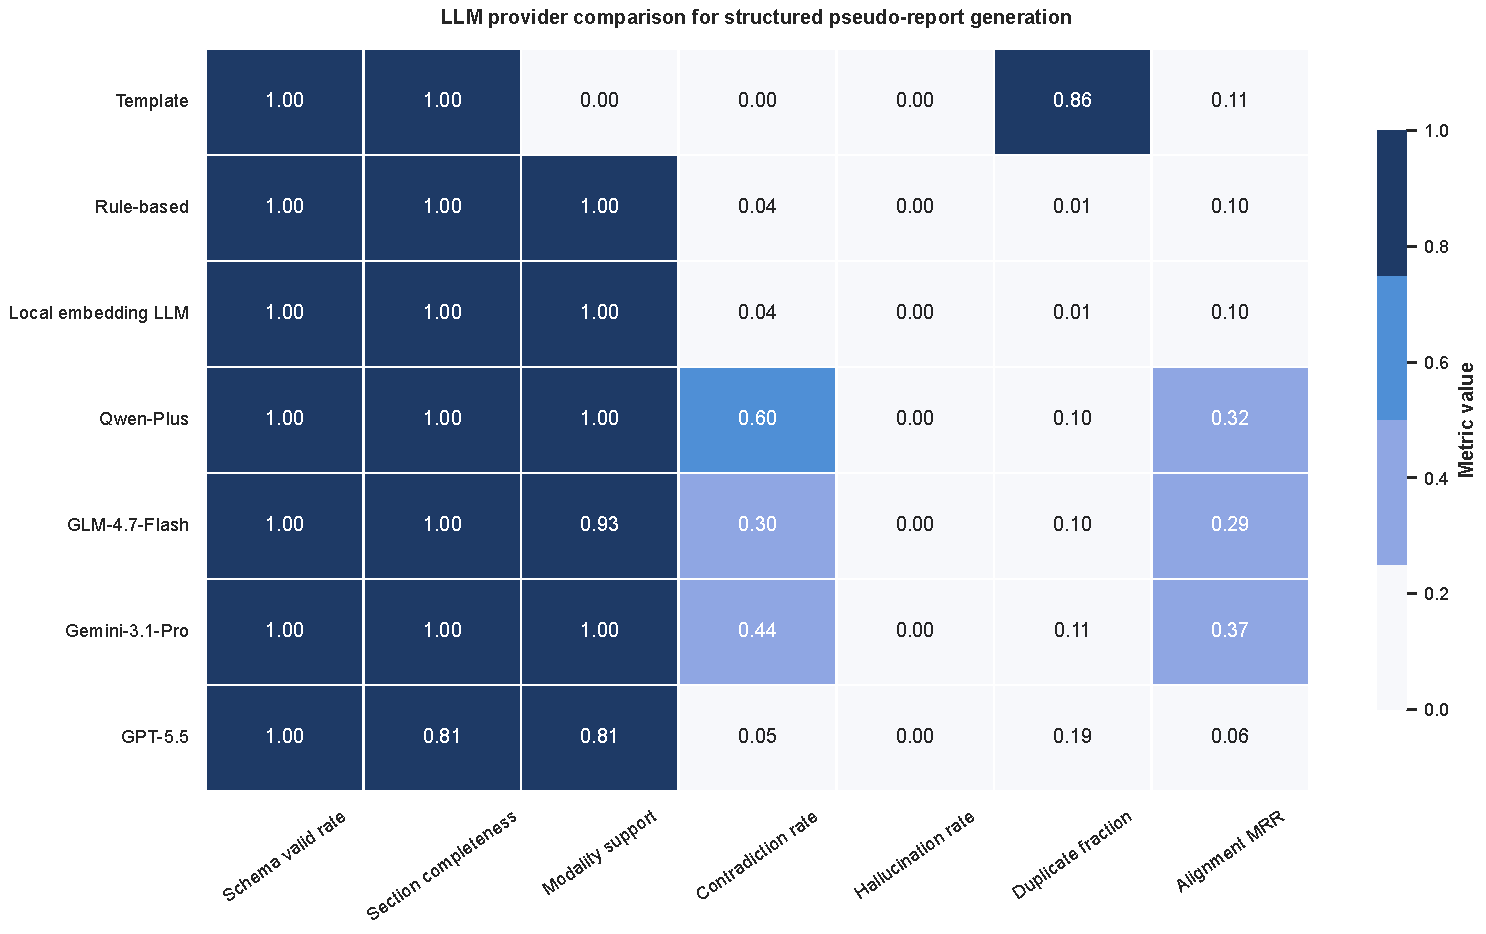
\includegraphics[width=\linewidth]{final_Fig/P8_llm_provider_comparison_heatmap.pdf}
  \caption{Supplementary provider-level comparison for structured pseudo-report generation. The heatmap summarises schema adherence, section completeness, modality support, contradiction risk, duplication, alignment, latency, and cost across template, rule-based, local LLM, and external API-based sources.}
  \label{fig:api_provider_summary_heatmap}
\end{figure}

\section*{Stage 1 pseudo-report quality and risk diagnostics}
\begin{figure}[!htbp]
  \centering
  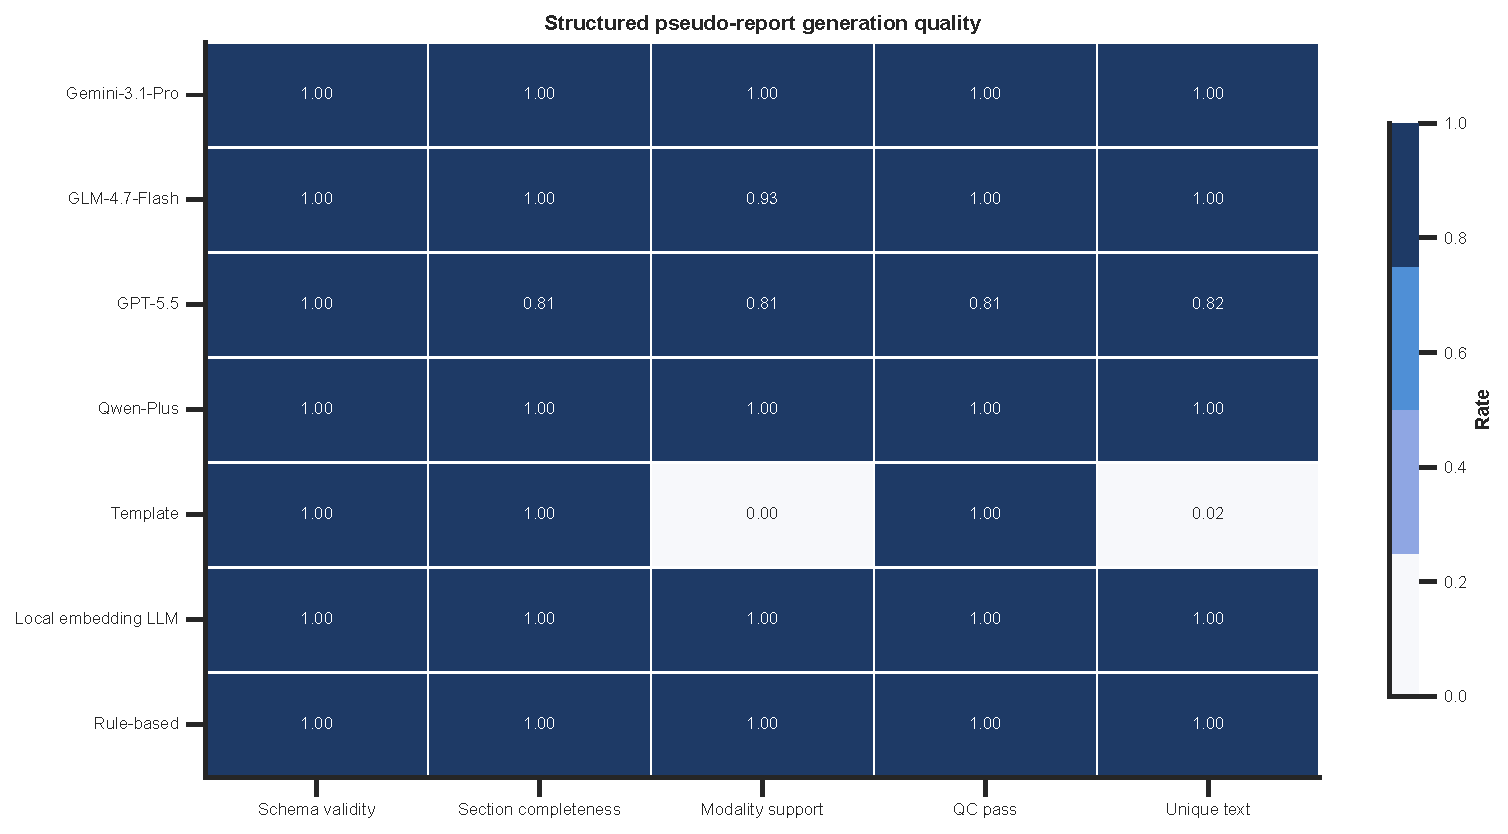
\includegraphics[width=\linewidth]{final_Fig/P1_stage1_quality_heatmap.pdf}
  \hfill
  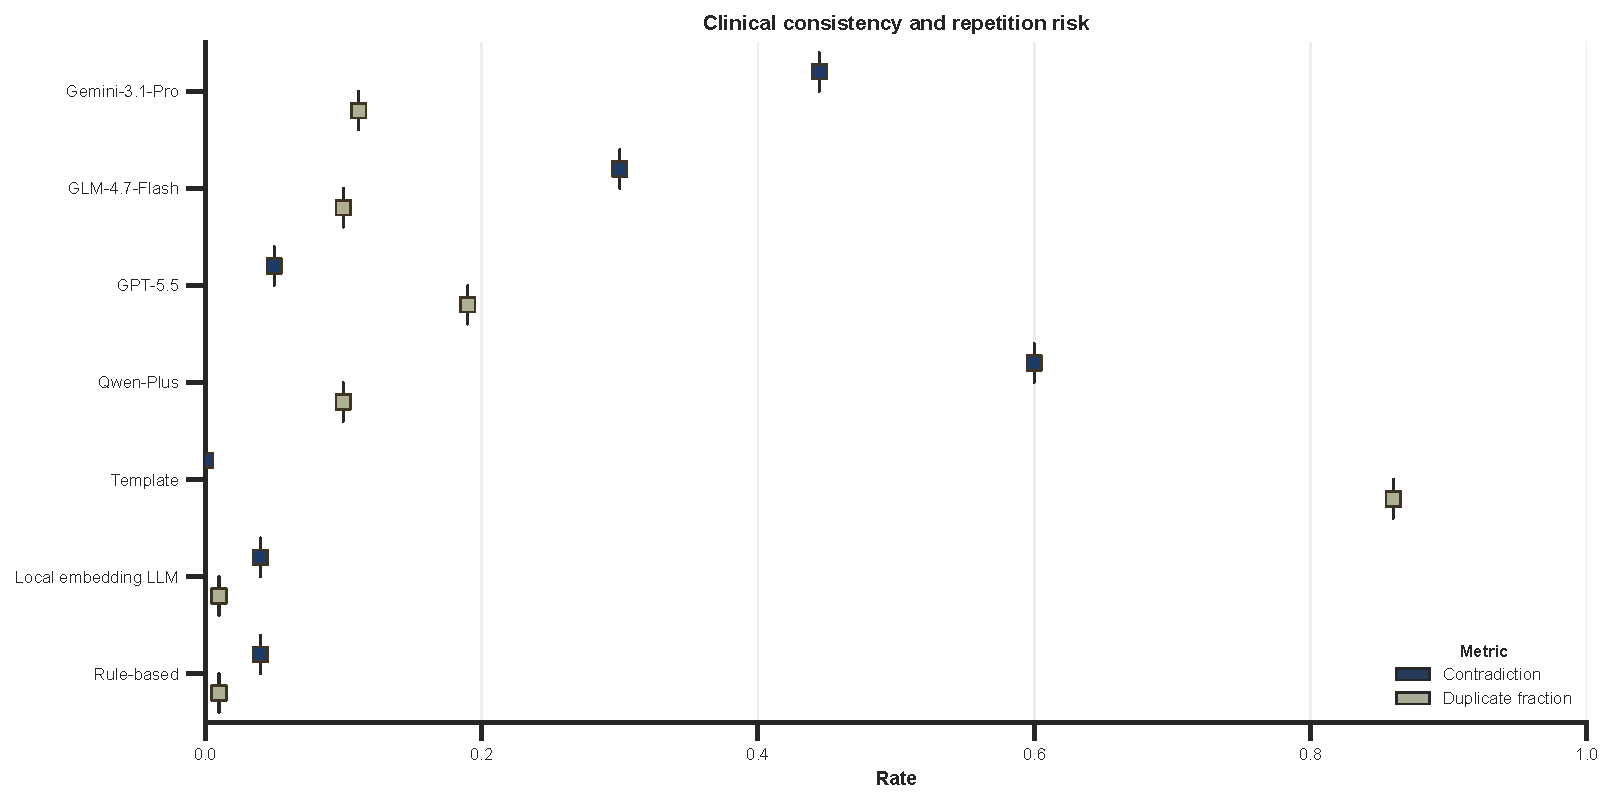
\includegraphics[width=\linewidth]{final_Fig/P2_stage1_quality_risk_bars.pdf}
  \caption{Supplementary Stage 1 evaluation of pseudo-report generation quality across LLM providers. The panels summarise generation validity and completeness together with risk-oriented quality indicators, including modality support, contradiction rate, hallucination rate, and duplicate-text behaviour.}
  \label{fig:api_quality_heatmap}
\end{figure}

\section*{Operational reliability of external pseudo-report generation}
\begin{figure}[!htbp]
  \centering
  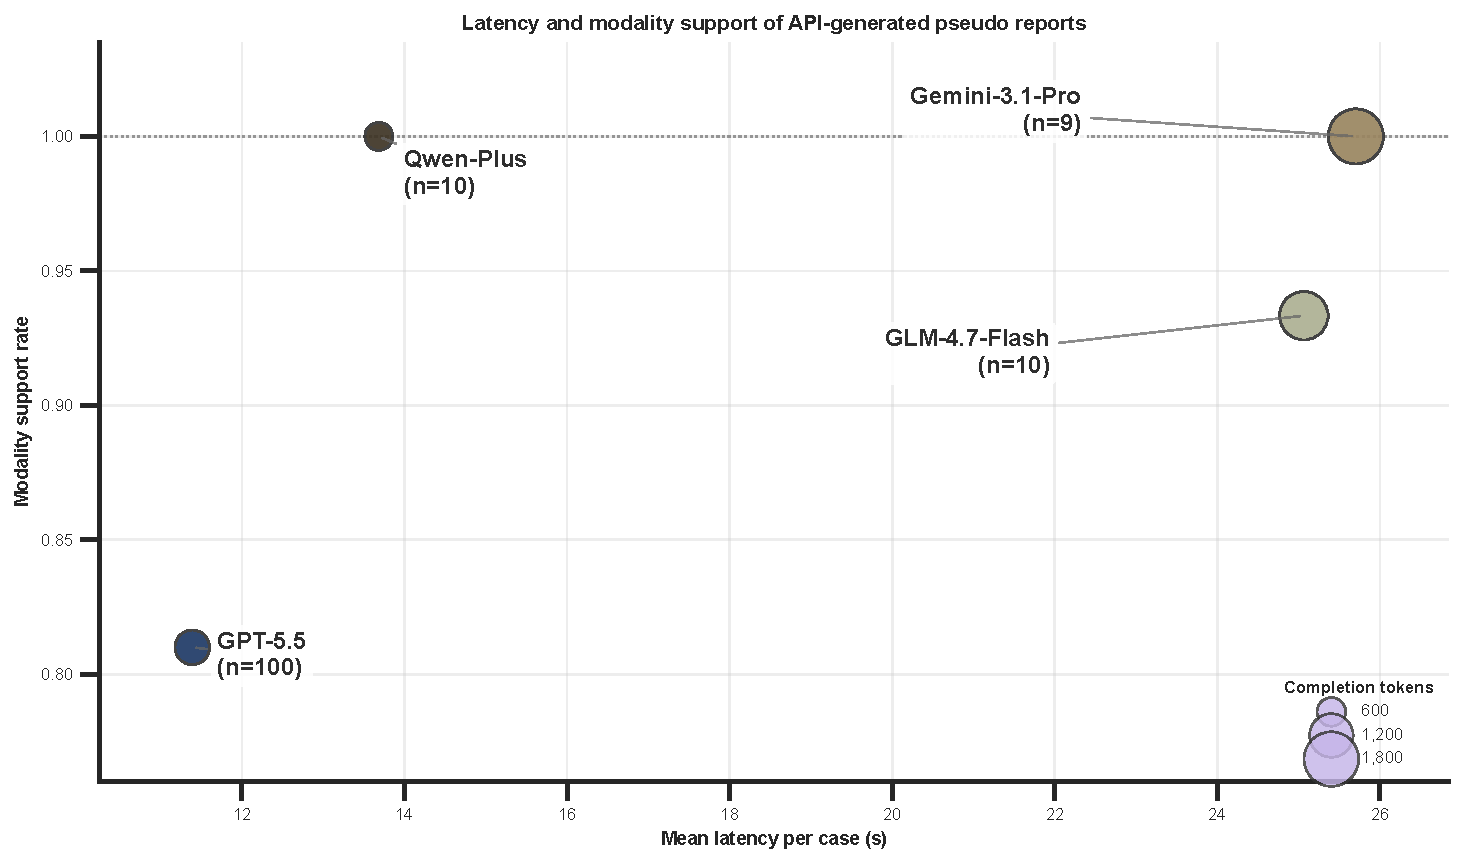
\includegraphics[width=\linewidth]{final_Fig/P3_stage1_latency_support_scatter.pdf}
  \hfill
  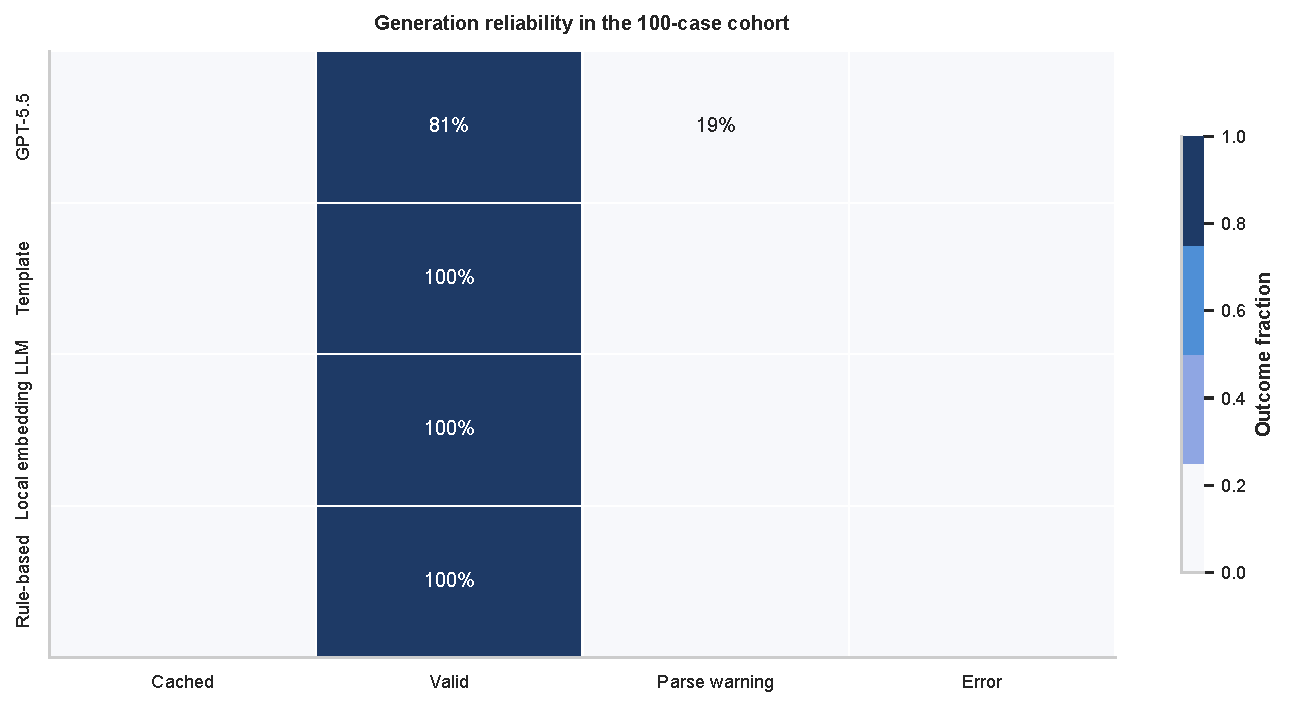
\includegraphics[width=\linewidth]{final_Fig/P4_stage1_generation_reliability.pdf}
  \caption{Supplementary operational reliability of external pseudo-report generation. The panels relate generation latency to modality support and summarise request completion and schema-valid output rates across evaluated providers.}
  \label{fig:api_reliability}
\end{figure}

\section*{Provider-generated pseudo reports in modality-section retrieval}
\begin{figure}[!htbp]
  \centering
  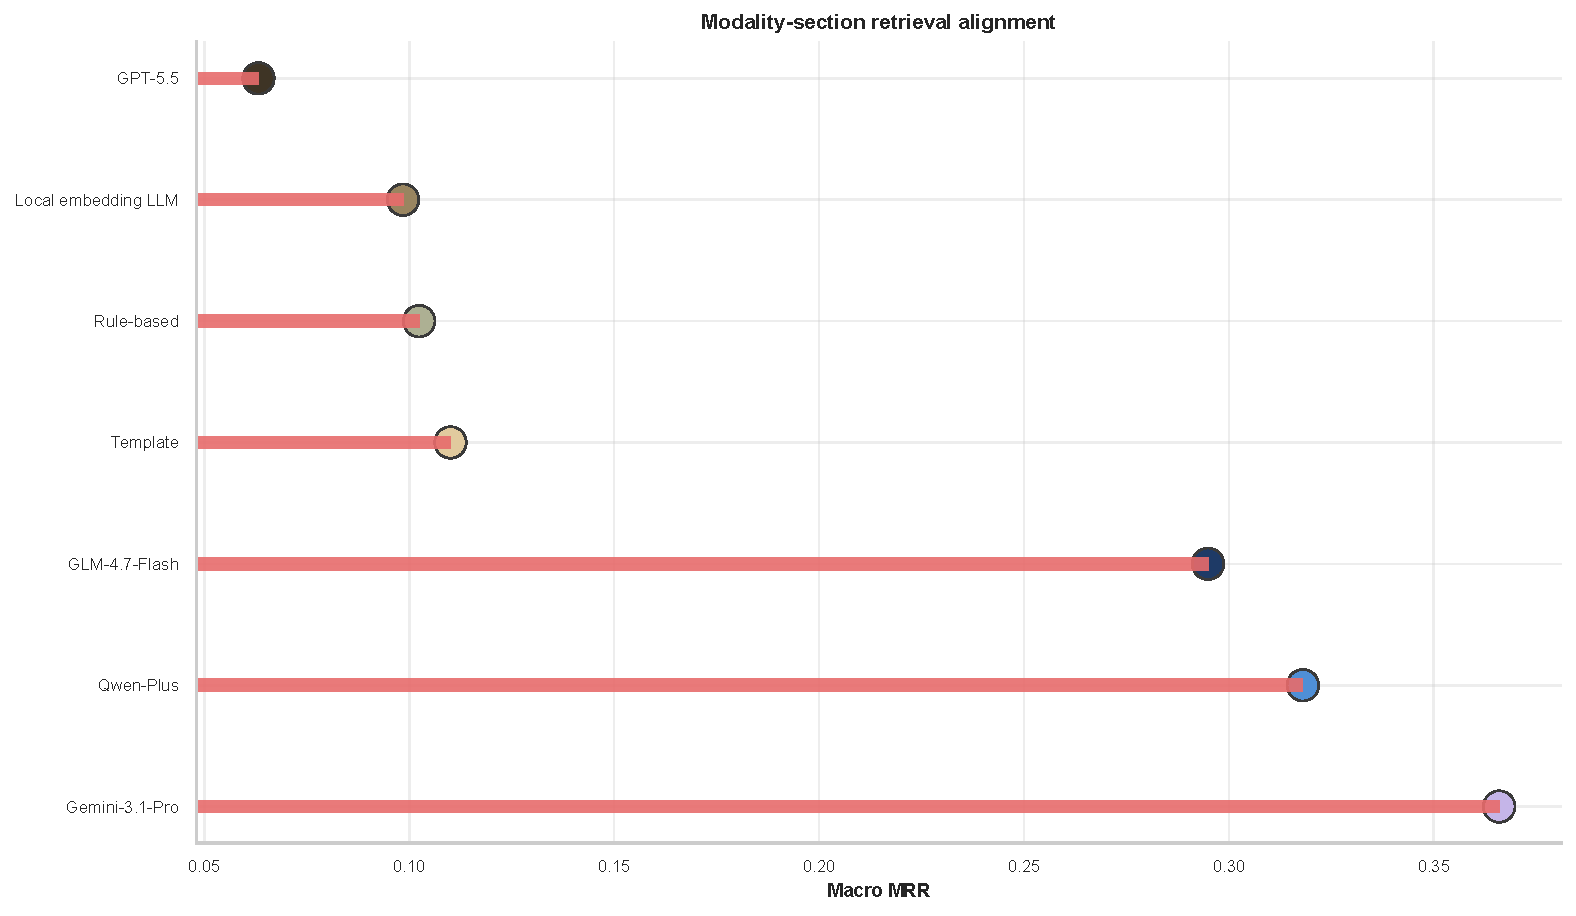
\includegraphics[width=\linewidth]{final_Fig/P5_stage2_macro_mrr.pdf}
  \hfill
  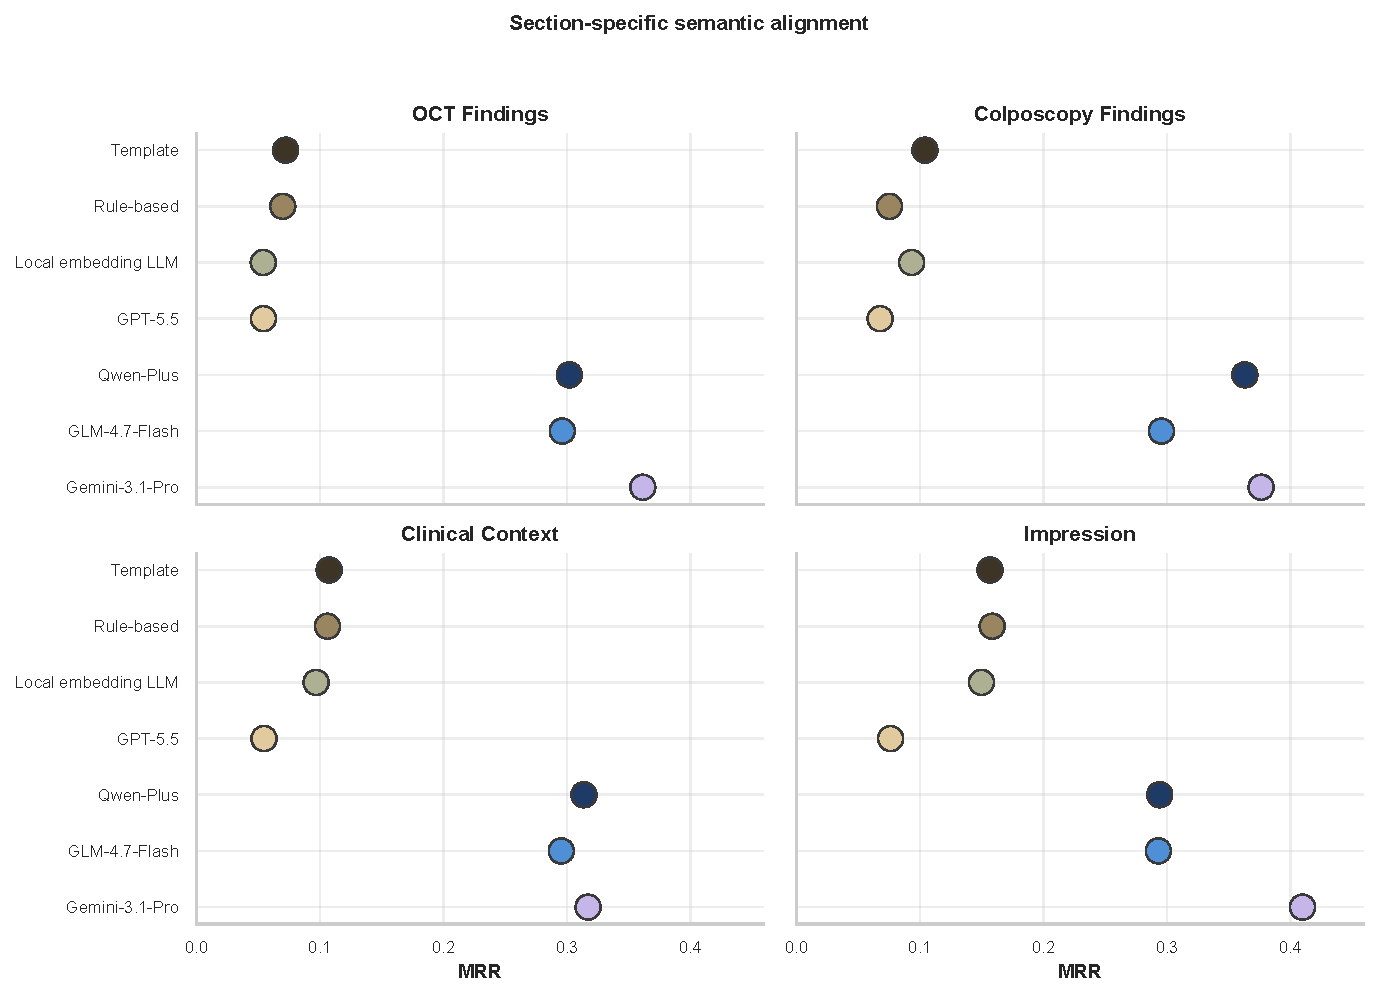
\includegraphics[width=\linewidth]{final_Fig/P6_stage2_section_mrr.pdf}
  \caption{Supplementary Stage 2 alignment evaluation for provider-generated pseudo reports. Macro MRR and section-specific MRR quantify how well report sections generated by different sources support modality-section semantic retrieval.}
  \label{fig:api_alignment_mrr}
\end{figure}

\section*{Section-specific retrieval performance across providers}
\begin{figure}[!htbp]
  \centering
  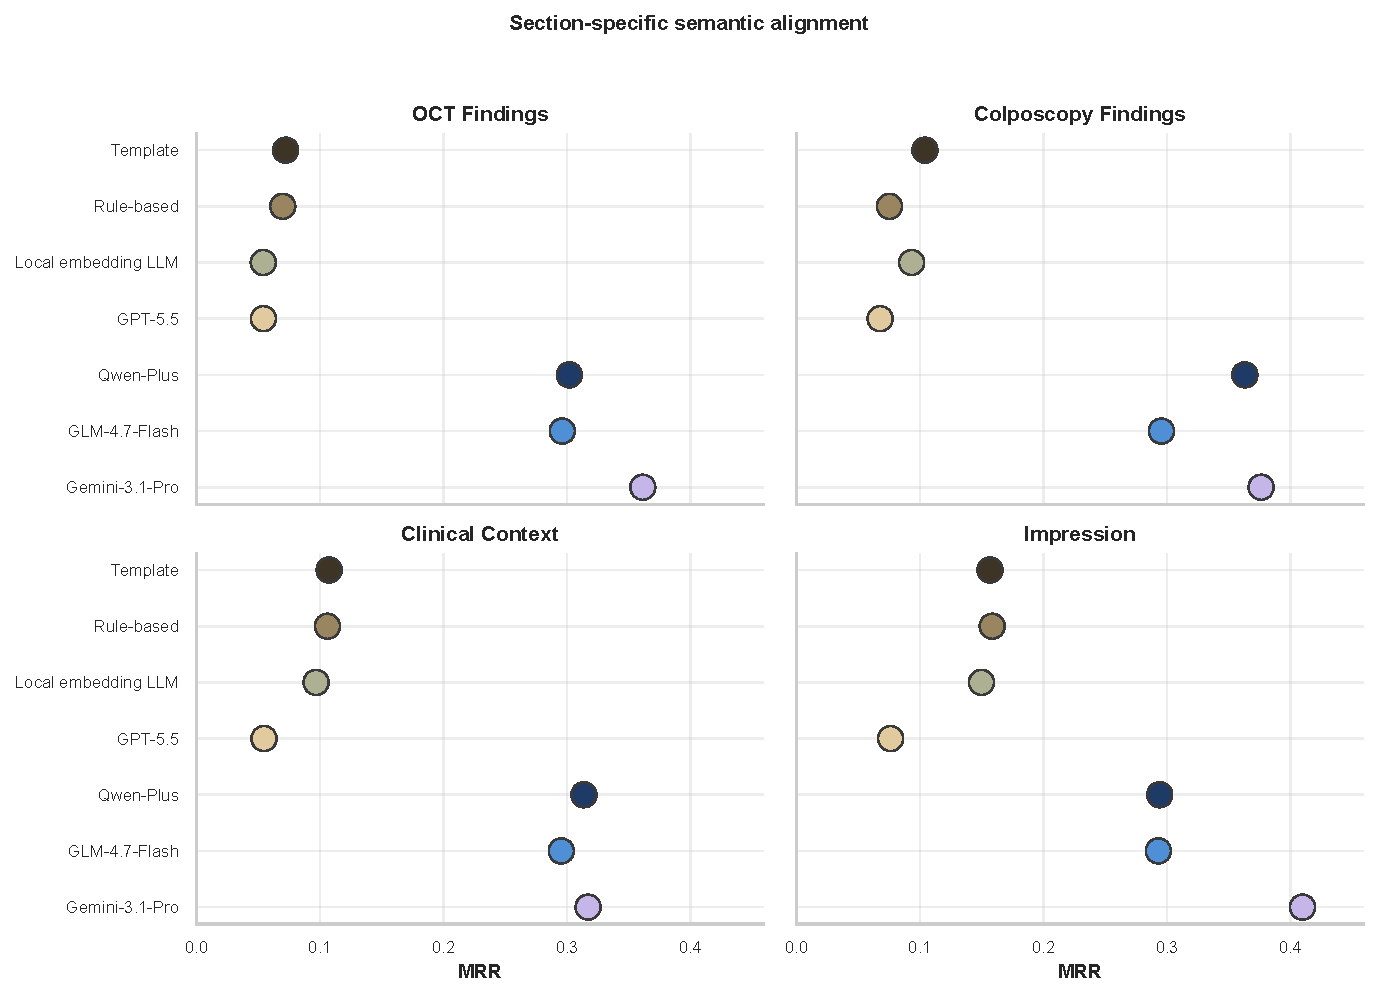
\includegraphics[width=\linewidth]{final_Fig/P6_stage2_section_mrr.pdf}
  \caption{Supplementary section-specific retrieval performance across pseudo-report providers. The analysis separately evaluates alignment for OCT findings, colposcopy findings, clinical context, and impression sections.}
  \label{fig:api_section_mrr}
\end{figure}

\section*{Downstream scarcity surrogate for API-generated pseudo reports}
\begin{figure}[!htbp]
  \centering
  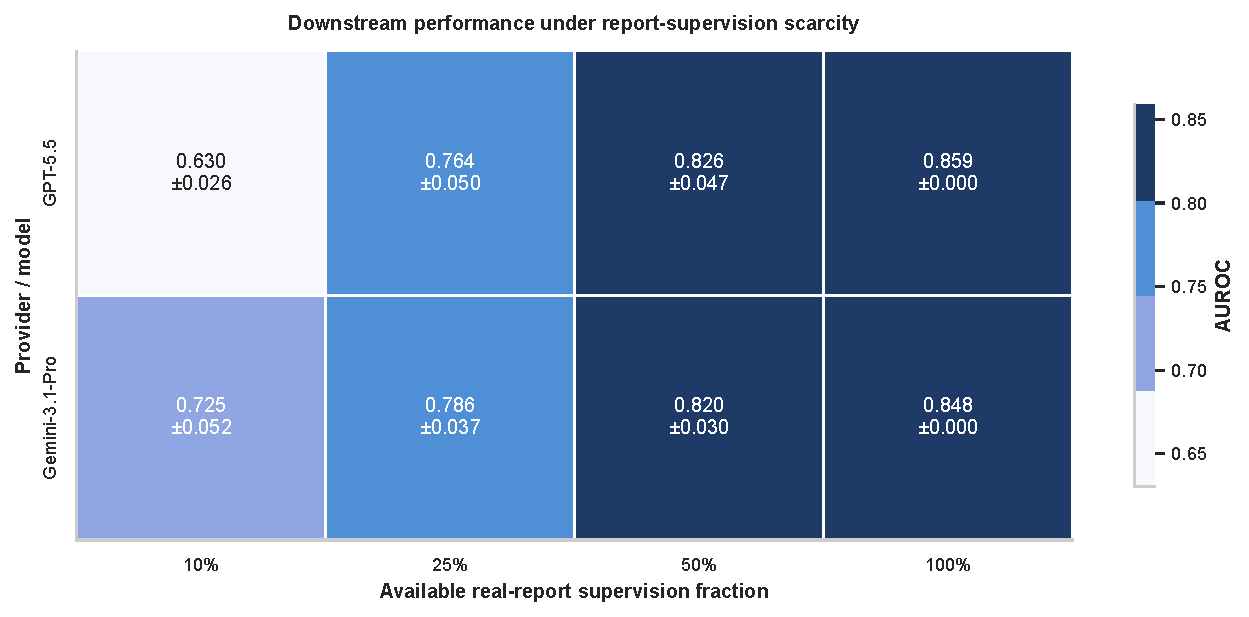
\includegraphics[width=\linewidth]{final_Fig/P7_stage3_scarcity_auc.pdf}
  \caption{Supplementary Stage 3 downstream scarcity surrogate using selected API-generated pseudo reports. The figure compares performance under reduced real-report supervision and evaluates whether externally generated structured reports provide useful supervision in low-report regimes.}
  \label{fig:api_scarcity_auc}
\end{figure}

\section*{Protocol harmonisation for pre-retrieval backbone results}
\begin{table*}[!htbp]
  \centering
  \caption{Supplementary protocol-harmonisation table. Pre-retrieval-calibration held-out test performance at validation-selected thresholds.}
  \label{tab:main_comparison}
  \scriptsize
  \begin{threeparttable}
  \resizebox{\linewidth}{!}{%
  \begin{tabular}{lrrr}
    \toprule
    \textbf{Model} & \textbf{AUROC [95\% CI]} & \textbf{F1 [95\% CI]} & \textbf{Threshold} \\
    \midrule
    \textbf{MOSAIC-RASA backbone} & \textbf{0.832} [0.757, 0.897] & \textbf{0.611} [0.458, 0.737] & 0.37 \\
    LCAD w/o section alignment     & \underline{0.826} [0.749, 0.894] & 0.510 [0.381, 0.624] & 0.24 \\
    Pseudo-augmented LCAD          & \underline{0.826} [0.747, 0.894] & \underline{0.545} [0.395, 0.674] & 0.39 \\
    Fusion w/o report anchor       & 0.802 [0.726, 0.873] & 0.457 [0.344, 0.557] & 0.16 \\
    Image-only report generator    & 0.763 [0.685, 0.837] & 0.453 [0.339, 0.553] & 0.17 \\
    Real-report only               & 0.725 [0.640, 0.801] & 0.356 [0.263, 0.438] & 0.14 \\
    Simple concatenation fusion    & 0.672 [0.584, 0.763] & 0.465 [0.380, 0.550] & 0.05 \\
    Instruction-only report generator & 0.630 [0.547, 0.717] & 0.459 [0.394, 0.519] & 0.14 \\
    \bottomrule
  \end{tabular}%
  }
  \begin{tablenotes}[flushleft]
    \footnotesize
    \item All models were evaluated on the same locked held-out test set ($n=288$). The repeated $n$ column was removed and reported here.
  \end{tablenotes}
  \end{threeparttable}
\end{table*}

\section*{MOSAIC metric profile for retrieval-calibrated fusion}
\begin{figure}[!htbp]
  \centering
  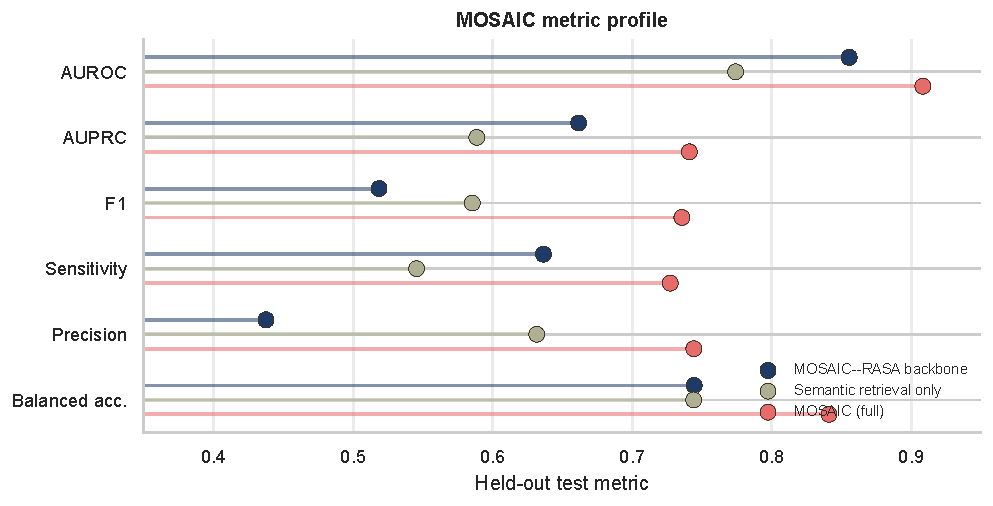
\includegraphics[width=\linewidth]{final_Fig/Figure_mosaic_metrics_heatmap.pdf}
  \caption{Supplementary compact metric heatmap for MOSAIC. The heatmap compares the MOSAIC-RASA backbone, retrieval-only semantic priors, and MOSAIC across discrimination and threshold-dependent metrics.}
  \label{fig:mosaic_metrics_heatmap}
\end{figure}

\section*{Historical report-aware backbone AUROC comparison}
\begin{figure}[!htbp]
  \centering
  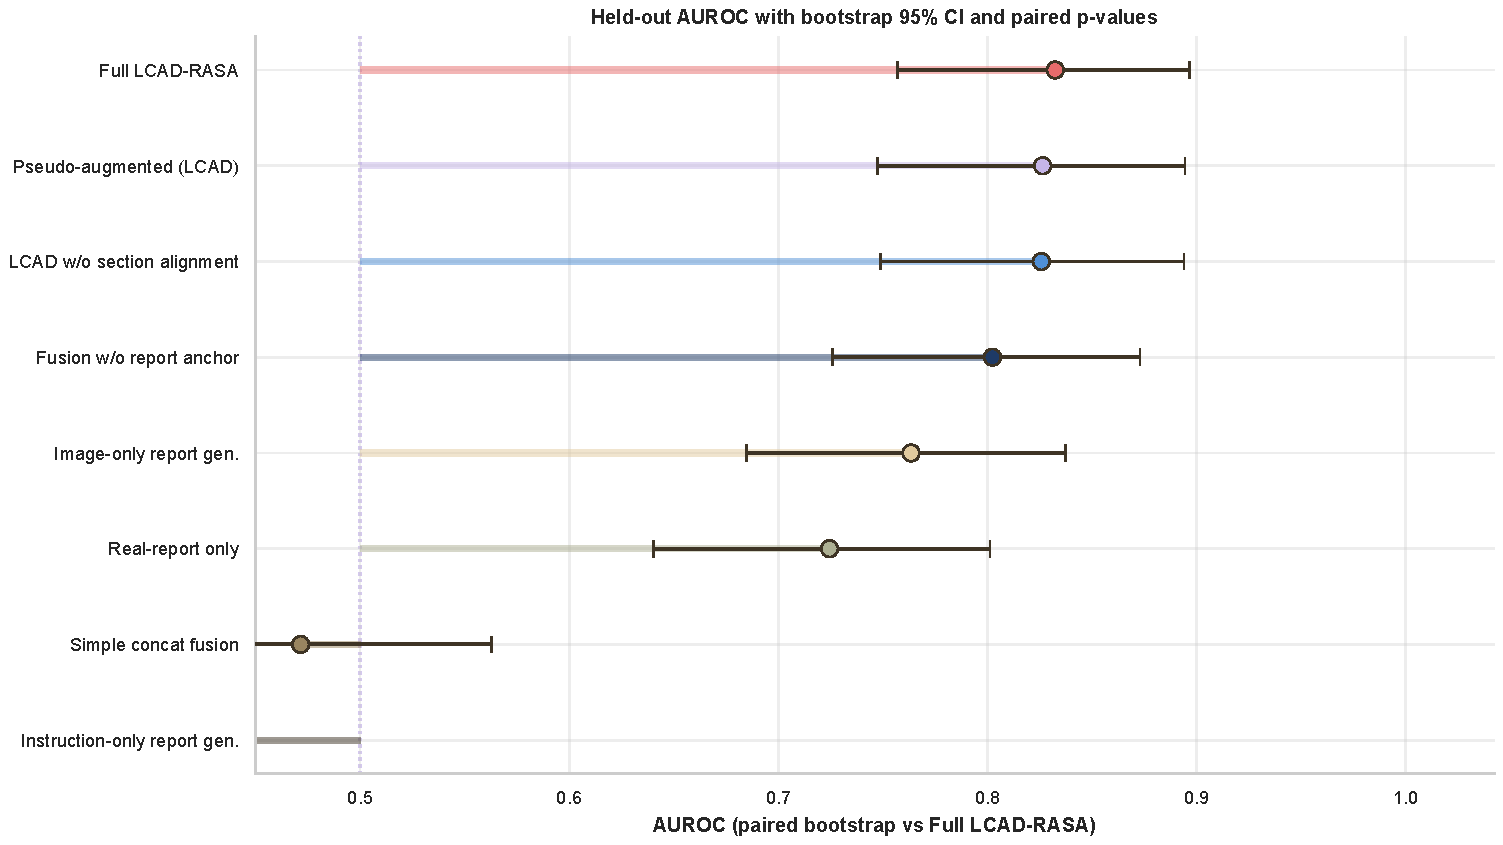
\includegraphics[width=\linewidth]{final_Fig/Figure_main_AUC_pointplot.pdf}
  \caption{Supplementary protocol-harmonisation plot. Held-out AUROC of report-aware backbone variants under the locked retrospective protocol. Points indicate test-set AUROC and intervals denote bootstrap 95\% confidence intervals.}
  \label{fig:main_auc}
\end{figure}

\section*{Multi-metric profile of historical backbone variants}
\begin{figure}[!htbp]
  \centering
  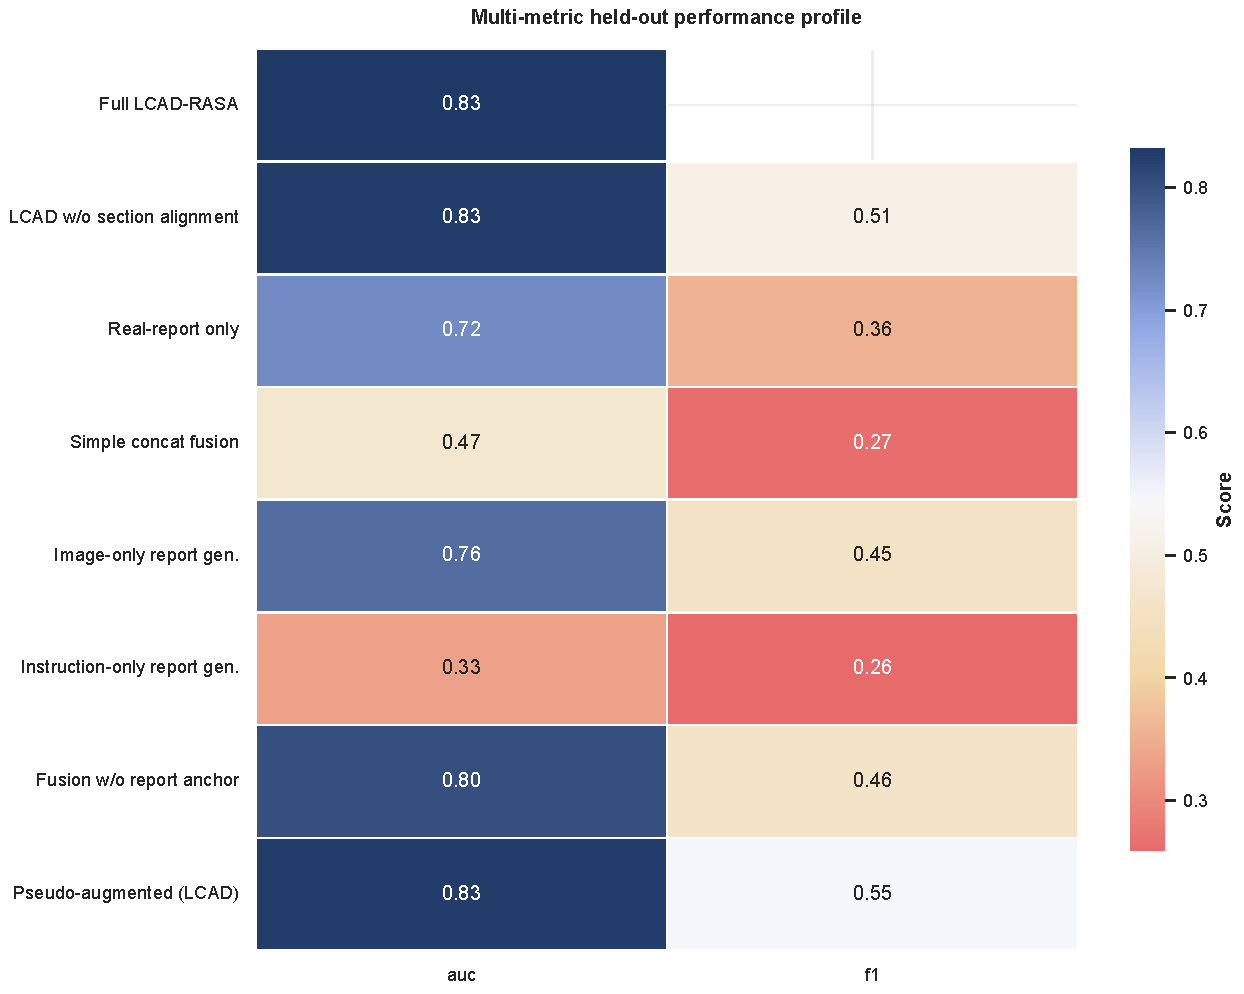
\includegraphics[width=\linewidth]{final_Fig/Figure_main_metrics_heatmap.pdf}
  \caption{Supplementary multi-metric held-out performance profile across historical backbone variants. The heatmap summarises discrimination, threshold-dependent performance, report consistency, and related evaluation metrics under the same locked test protocol.}
  \label{fig:main_metrics}
\end{figure}

\section*{AUROC--F1 trade-off among backbone variants}
\begin{figure}[!htbp]
  \centering
  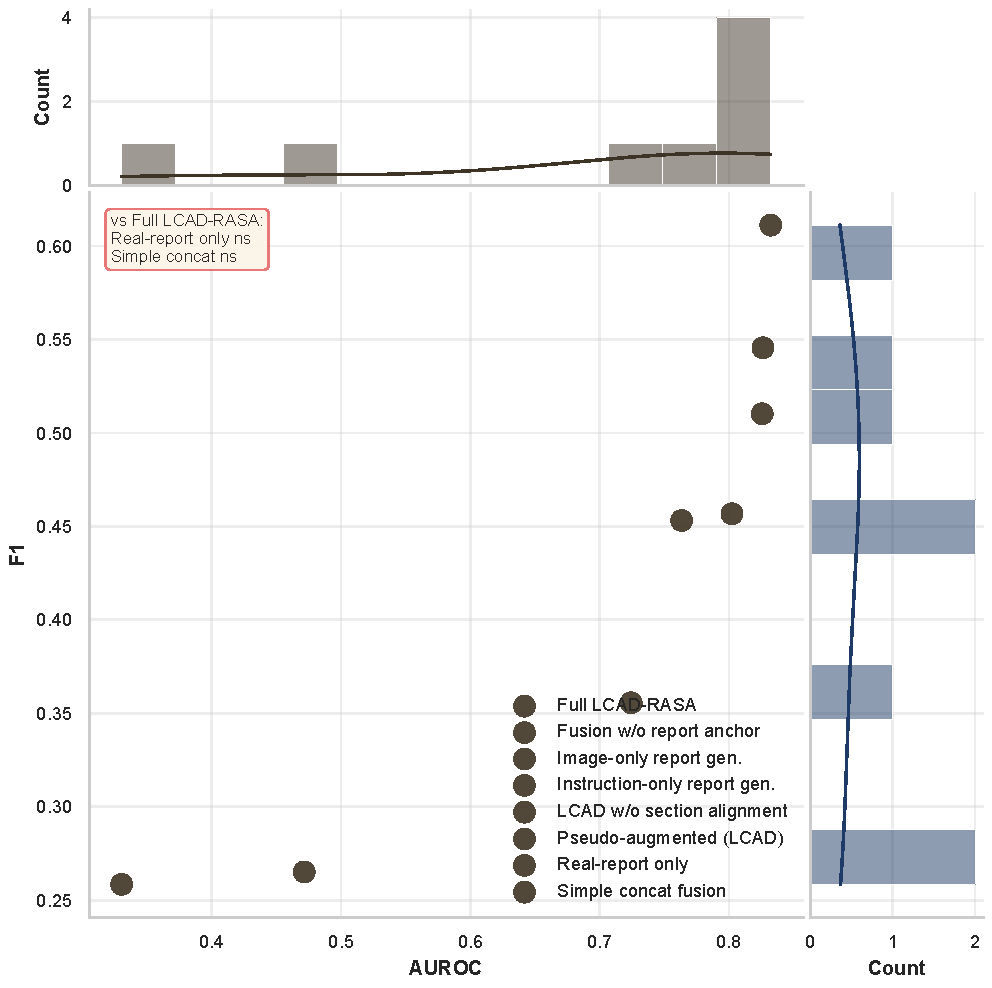
\includegraphics[width=\linewidth]{final_Fig/Figure_main_auc_f1_scatter.pdf}
  \caption{Supplementary AUROC--F1 operating trade-off across historical backbone variants. The scatter plot contrasts rank-based discrimination with threshold-dependent classification performance on the held-out test set.}
  \label{fig:main_auc_f1}
\end{figure}

\section*{LLM-specific semantic-tag availability and retrieval ablation}
\begin{table*}[!htbp]
  \centering
  \caption{Supplementary Table S4a. LLM-specific semantic-tag and retrieval ablation.}
  \label{tab:llm_specific_ablation}
  \scriptsize
  \begin{threeparttable}
  \resizebox{\linewidth}{!}{%
  \begin{tabular}{lcccrrrrrrr}
    \toprule
    \textbf{Method} & \textbf{Uses LLM} & \textbf{\makecell{Train-only\\bank}} & \textbf{\makecell{Validation\\fusion}} & \textbf{AUROC} & \textbf{AUPRC} & \textbf{F1} & \textbf{Sensitivity} & \textbf{Specificity} & \textbf{$\alpha$} & \textbf{Threshold} \\
    \midrule
    MOSAIC-RASA backbone only & No & \NA & Threshold only & 0.856 & 0.662 & 0.519 & 0.636 & 0.852 & \NA & 0.39 \\
    Clean rule-tag retrieval only & No & Yes & Threshold only & 0.724 & 0.349 & 0.480 & 0.682 & 0.791 & \NA & 0.30 \\
    MOSAIC-Tag: RASA + clean rule-tag fusion & No & Yes & Yes & 0.878 & 0.695 & 0.556 & 0.568 & 0.914 & 0.10 & 0.40 \\
    LLM-tag retrieval only & Yes & Yes & Threshold only & \NA & \NA & \NA & \NA & \NA & \NA & \NA \\
    RASA + LLM-tag retrieval fusion & Yes & Yes & Yes & \NA & \NA & \NA & \NA & \NA & \NA & \NA \\
    RASA + LLM-tag fusion + verifier weighting & Yes & Yes & Yes & \NA & \NA & \NA & \NA & \NA & \NA & \NA \\
    MOSAIC & Indirect & Yes & Yes & 0.908 & 0.741 & 0.736 & 0.727 & 0.955 & \NA & 0.50 \\
    CLIP-style contrastive baseline & No & \NA & Threshold only & 0.888 & 0.739 & 0.640 & 0.545 & 0.971 & \NA & 0.79 \\
    \bottomrule
  \end{tabular}%
  }
  \begin{tablenotes}[flushleft]
    \footnotesize
    \item LLM-tag rows are unavailable because no valid LLM semantic tag table was generated in the current run. Rule-tag rows are deterministic fallback audits and must not be interpreted as LLM evidence. All available tag-retrieval rows used a cleaned training-only bank; fusion weights and thresholds were selected on validation data only. MOSAIC-Tag is a secondary semantic-tag audit rather than the primary MOSAIC model.
  \end{tablenotes}
  \end{threeparttable}
\end{table*}

\section*{Cleaned semantic-tag source ablations and negative controls}
\begin{table*}[!htbp]
  \centering
  \caption{Supplementary Table S4b. Cleaned semantic-tag source ablation and negative controls.}
  \label{tab:semantic_tag_source_ablation_cleaned}
  \scriptsize
  \begin{threeparttable}
  \resizebox{\linewidth}{!}{%
  \begin{tabular}{lrrrrp{4.2cm}}
    \toprule
    \textbf{Variant} & \textbf{\makecell{Retrieval-only\\AUROC}} & \textbf{\makecell{Fusion\\AUROC}} & \textbf{\(\Delta\)AUROC vs RASA} & \textbf{\makecell{95\% interval}} & \textbf{Interpretation} \\
    \midrule
    MOSAIC-Tag, all clean rule tags & 0.724 & 0.878 & 0.023 & 0.003--0.042 & Cleaned semantic-tag audit; secondary analysis \\
    No impression tags & 0.724 & 0.878 & 0.023 & 0.003--0.042 & No loss after removing impression-tag column \\
    No severity tags & 0.724 & 0.878 & 0.023 & 0.003--0.042 & No loss after removing severity-tag column \\
    No diagnostic terminology & 0.724 & 0.878 & 0.023 & 0.003--0.042 & Effect persisted after diagnostic-term removal \\
    Modality-only or visual-only tags & 0.500 & 0.856 & 0.000 & 0.000--0.000 & Collapsed to MOSAIC-RASA backbone \\
    Train-label prior only & 0.500 & 0.856 & 0.000 & 0.000--0.000 & Negative control did not improve over backbone \\
    Random tag query & 0.462 & 0.853 & -0.002 & -0.006--0.002 & Random-query negative control removed the tag gain \\
    Random train-label bank & 0.582 & 0.856 & 0.000 & 0.000--0.000 & Label-permutation control removed the tag gain \\
    Same-centre excluded retrieval & 0.628 & 0.864 & 0.008 & -0.003--0.019 & Cross-centre retrieval retained limited signal but was weaker \\
    \bottomrule
  \end{tabular}%
  }
  \begin{tablenotes}[flushleft]
    \footnotesize
    \item All rows used the semantic-tag audit protocol: cleaned tag input, training-only tag bank, validation-selected fusion weight and threshold, and locked held-out test metrics. MOSAIC-Tag passed leakage screening and negative controls, but its role is a lightweight semantic-prior audit rather than a replacement for MOSAIC.
  \end{tablenotes}
  \end{threeparttable}
\end{table*}

\section*{RASA alignment-weight sensitivity}
\begin{table}[!htbp]
  \centering
  \caption{Supplementary Table S1. RASA alignment-weight sweep.}
  \label{tab:s1_rasa_lambda_align_sweep}
  \small
  \begin{threeparttable}
  \begin{tabular}{lr}
    \toprule
    \textbf{$\lambda_{\mathrm{align}}$} & \textbf{AUROC} \\
    \midrule
    0.00 & 0.766 \\
    0.01 & 0.766 \\
    0.05 & 0.769 \\
    0.10 & 0.773 \\
    0.20 & \textbf{0.776} \\
    0.50 & 0.772 \\
    1.00 & 0.764 \\
    \bottomrule
  \end{tabular}
  \begin{tablenotes}[flushleft]
    \footnotesize
    \item F1 was 0.451, label consistency was 0.641, and section completeness was 1.000 for all settings; these constant columns were omitted.
  \end{tablenotes}
  \end{threeparttable}
\end{table}

\section*{Input-modality ablation}
\begin{table*}[!htbp]
  \centering
  \caption{Supplementary Table S3. Modality ablation.}
  \label{tab:s3_modality_ablation}
  \small
  \begin{threeparttable}
  \resizebox{\linewidth}{!}{%
  \begin{tabular}{lrrrr}
    \toprule
    \textbf{Variant} & \textbf{AUROC} & \textbf{F1} & \textbf{Sensitivity} & \textbf{Specificity} \\
    \midrule
    Colposcopy + clinical instruction        & \textbf{0.850} & 0.524 & \underline{0.614} & 0.869 \\
    Full without fused visual embedding      & \underline{0.840} & \underline{0.571} & 0.500 & \textbf{0.955} \\
    OCT + colposcopy + clinical instruction  & \underline{0.840} & \underline{0.571} & 0.500 & \textbf{0.955} \\
    Colposcopy only                          & 0.838 & \textbf{0.581} & \underline{0.614} & 0.910 \\
    Full with fused visual embedding         & 0.836 & 0.561 & 0.523 & 0.939 \\
    OCT + colposcopy                         & 0.826 & 0.543 & 0.568 & 0.906 \\
    OCT + clinical instruction               & 0.765 & 0.466 & 0.386 & \underline{0.951} \\
    OCT only                                 & 0.740 & 0.353 & 0.409 & 0.836 \\
    Clinical instruction only                & 0.683 & 0.441 & \textbf{0.727} & 0.717 \\
    \bottomrule
  \end{tabular}%
  }
  \begin{tablenotes}[flushleft]
    \footnotesize
    \item Label consistency was 0.641 for all modality variants and was removed as a constant column.
  \end{tablenotes}
  \end{threeparttable}
\end{table*}

\section*{LCAD pseudo-report quality-control ablation}
\begin{table}[!htbp]
  \centering
  \caption{Supplementary Table S4. LCAD pseudo-report quality-control ablation.}
  \label{tab:s4_lcad_qc_ablation}
  \small
  \begin{threeparttable}
  \begin{tabular}{lrrrr}
    \toprule
    \textbf{QC strategy} & \textbf{AUROC} & \textbf{F1} & \textbf{Sensitivity} & \textbf{Specificity} \\
    \midrule
    \makecell[l]{Pseudo reports, no QC;\\QC-pass pseudo reports only;\\QC-score weighting only;\\Pseudo confidence weighting only;\\QC-confidence weighted pseudo reports} & 0.836 & 0.561 & 0.523 & 0.939 \\
    \bottomrule
  \end{tabular}
  \begin{tablenotes}[flushleft]
    \footnotesize
    \item All QC variants produced identical downstream metrics under this retrospective configuration. Duplicate rows were therefore merged. Label consistency was 0.641 for all variants.
  \end{tablenotes}
  \end{threeparttable}
\end{table}

\section*{Failure-enriched pseudo-report QC stress test}
\begin{table}[!htbp]
  \centering
  \caption{Supplementary Table S4c. Failure-enriched QC stress-test v2 audit.}
  \label{tab:qc_failure_stress_test}
  \small
  \begin{threeparttable}
  \begin{tabular}{p{5.0cm}rp{5.2cm}}
    \toprule
    \textbf{Stress-test metric} & \textbf{Value} & \textbf{Interpretation} \\
    \midrule
    Clean pseudo-report QC pass rate & 1.000 & clean baseline retained \\
    Corrupted pseudo-report QC pass rate & 0.742 & corrupted variants partly rejected or down-weighted \\
    Mean QC score, clean vs corrupted & 1.000 vs 0.855 & corrupted reports down-weighted \\
    Severe-error flag rate, clean vs corrupted & 0.000 vs 0.258 & severe failures enriched among corrupted reports \\
    Contradiction detection rate & 1.000 & expected contradiction flags detected \\
    Hallucination detection rate & 0.999 & unsupported terminology or missing-modality evidence detected \\
    Missing-section detection rate & 1.000 & empty required sections detected \\
    Modality-swap detection rate & 1.000 & v2 modality--section consistency detector captured OCT--colposcopy swaps and shuffled sections \\
    Duplicate-template detection rate & 1.000 & repeated template text detected \\
    \bottomrule
  \end{tabular}
  \begin{tablenotes}[flushleft]
    \footnotesize
    \item The stress test used all 1,153 pseudo-report candidates and the v2 QC function. The clean modality-swap false-positive rate was 0.000. No retraining under corrupted reports was performed, and no LLM verifier comparison is claimed. Source files: \texttt{outputs/qc/qc\_stress\_test\_v2.csv}, \texttt{outputs/qc/qc\_stress\_test\_v2\_detail.csv}, and \texttt{outputs/qc/qc\_failure\_enriched\_stress\_test.png}.
  \end{tablenotes}
  \end{threeparttable}
\end{table}

\section*{RASA component ablation}
\begin{table*}[!htbp]
  \centering
  \caption{Supplementary Table S5. RASA component ablation.}
  \label{tab:s5_rasa_component_ablation}
  \small
  \begin{threeparttable}
  \resizebox{\linewidth}{!}{%
  \begin{tabular}{lrrrr}
    \toprule
    \textbf{Variant} & \textbf{AUROC} & \textbf{F1} & \textbf{Sensitivity} & \textbf{Specificity} \\
    \midrule
    Risk-head auxiliary only                 & \textbf{0.838} & 0.538 & \underline{0.568} & 0.902 \\
    No section alignment                     & \textbf{0.838} & 0.479 & \textbf{0.636} & 0.816 \\
    No label-consistency loss                & 0.836 & \textbf{0.579} & 0.500 & \textbf{0.959} \\
    MOSAIC-RASA backbone                    & 0.836 & \underline{0.561} & 0.523 & \underline{0.939} \\
    \makecell[l]{No risk head;\\Report loss only;\\Section alignment auxiliary only} & 0.750 & 0.465 & 0.550 & 0.820 \\
    \bottomrule
  \end{tabular}%
  }
  \begin{tablenotes}[flushleft]
    \footnotesize
    \item Label consistency was 0.641 for all component variants and was removed as a constant column. Three variants with identical metrics were merged into one row.
  \end{tablenotes}
  \end{threeparttable}
\end{table*}

\section*{Extended metric profiles for same-split baselines}
\begin{figure}[!htbp]
  \centering
  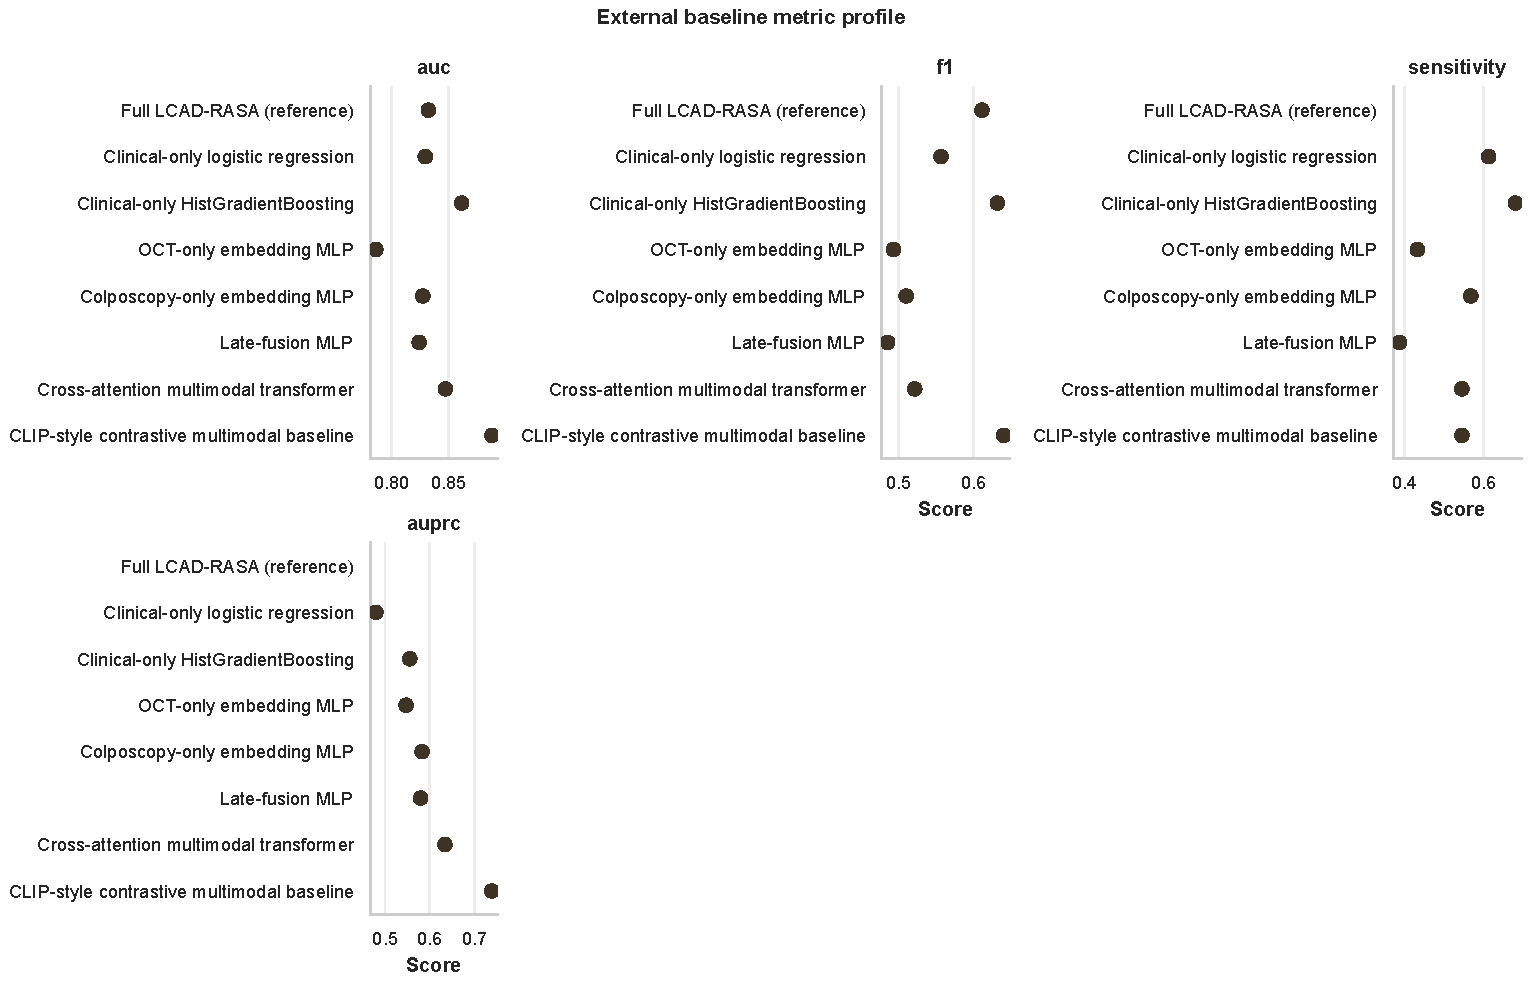
\includegraphics[width=\linewidth]{final_Fig/Figure_external_baselines_metric_dotplot.pdf}
  \caption{Supplementary metric profile of MOSAIC, the MOSAIC-RASA backbone, and external baselines under the locked held-out protocol. The dot plot compares discrimination and threshold-dependent metrics across clinical-only, image-only, late-fusion, cross-attention, contrastive, and report-aware models.}
  \label{fig:external_baselines_metrics}
\end{figure}

\section*{Corrected paired-bootstrap recheck against the backbone}
\begin{figure}[!htbp]
  \centering
  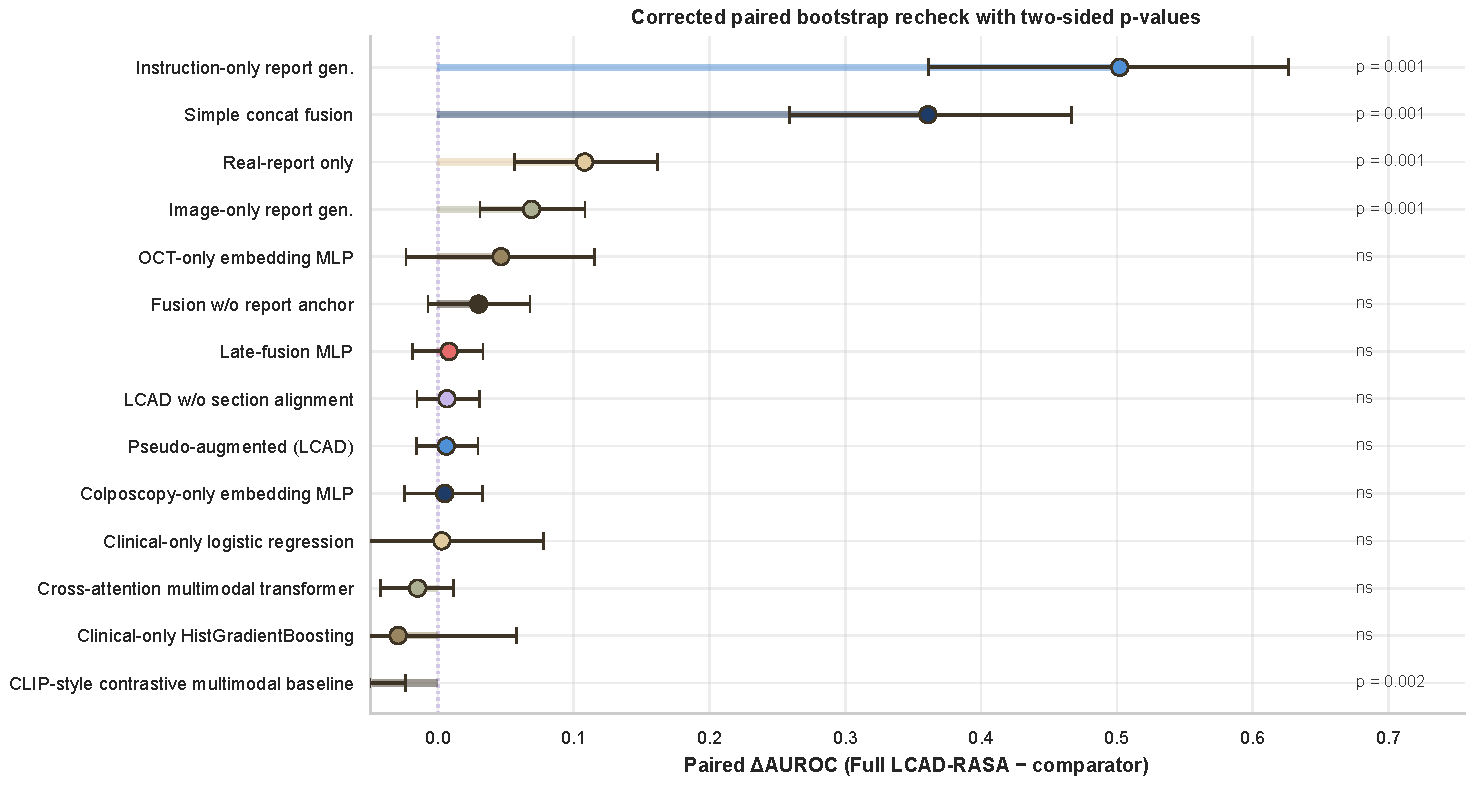
\includegraphics[width=\linewidth]{final_Fig/Figure_external_baselines_paired_delta_auc.pdf}
  \caption{Supplementary corrected paired bootstrap AUROC differences relative to the MOSAIC-RASA backbone. Positive values favour the backbone, whereas negative values favour the comparator, with intervals estimated from paired test-set resampling.}
  \label{fig:external_pairwise_recheck}
\end{figure}

\section*{Alignment-weight sensitivity visualisation}
\begin{figure}[!htbp]
  \centering
  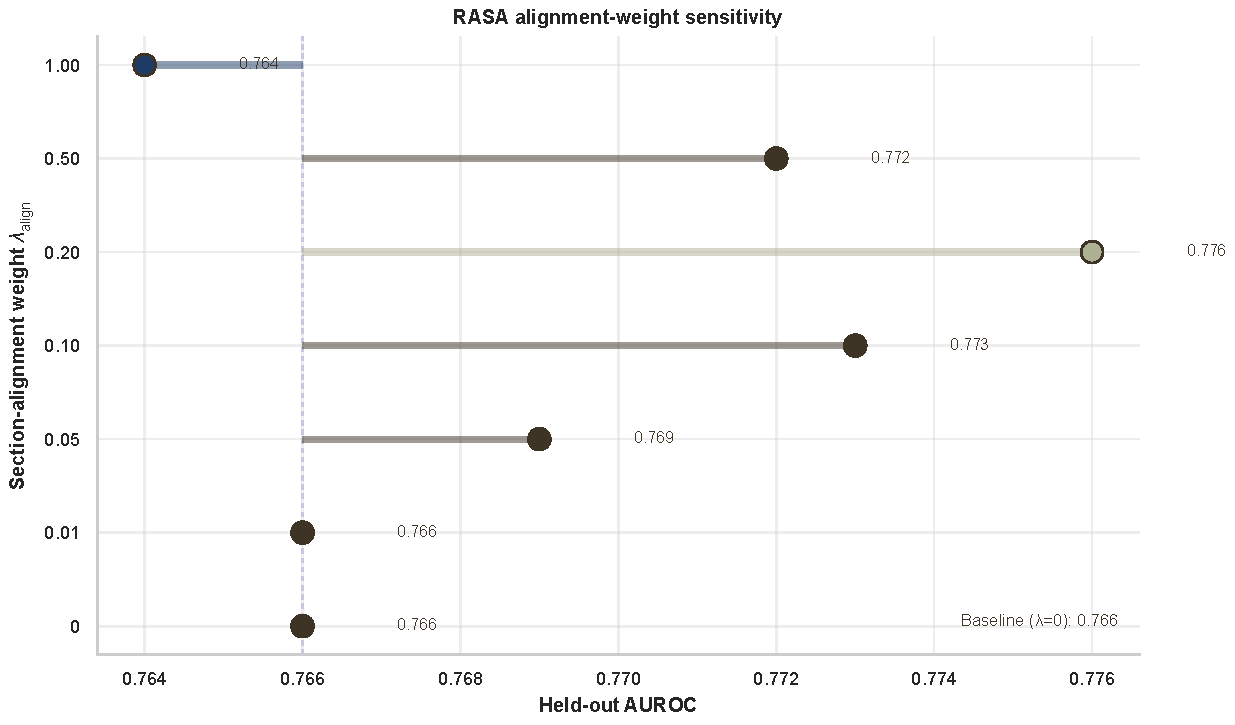
\includegraphics[width=\linewidth]{final_Fig/fig_rasa_lambda_lineplot.pdf}
  \caption{Supplementary sensitivity of model performance to the RASA alignment weight. The sweep evaluates how varying the section-alignment loss weight affects downstream discrimination and report-related metrics.}
  \label{fig:rasa_lambda}
\end{figure}

\section*{Joint modality and RASA component visual ablations}
\begin{figure}[!htbp]
  \centering
  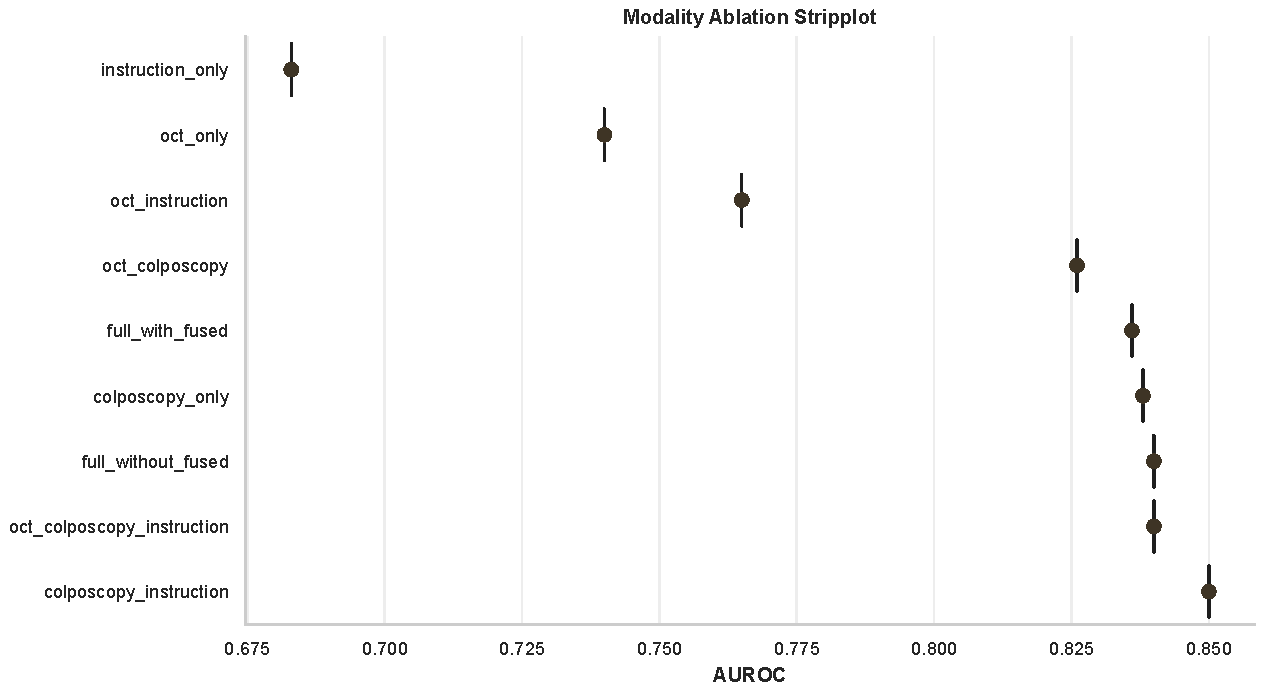
\includegraphics[width=\linewidth]{final_Fig/fig_modality_ablation_stripplot.pdf}
  \hfill
  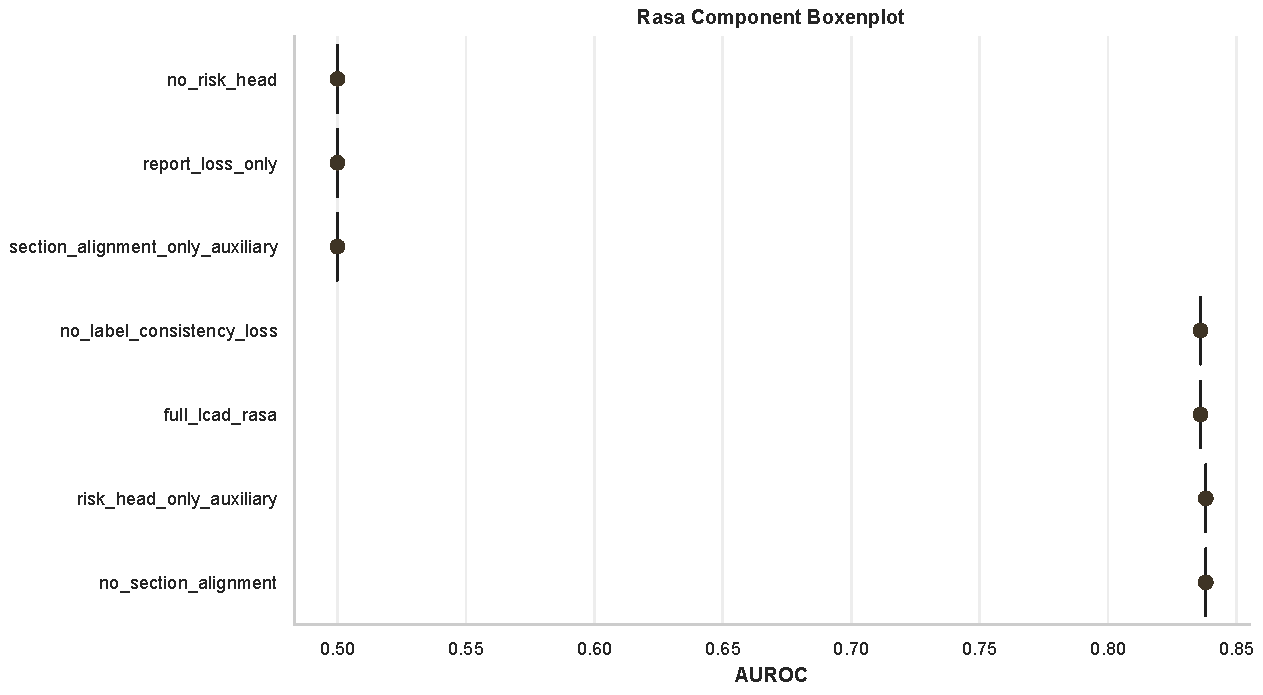
\includegraphics[width=\linewidth]{final_Fig/fig_rasa_component_boxenplot.pdf}
  \caption{Supplementary ablation analysis of modality inputs and RASA components. The panels assess the contribution of OCT, colposcopy, clinical instruction, fused visual embeddings, section alignment, risk supervision, and label-consistency terms.}
  \label{fig:rasa_component_boxenplot}
\end{figure}

\section*{LCAD quality-control ablation visualisation}
\begin{figure}[!htbp]
  \centering
  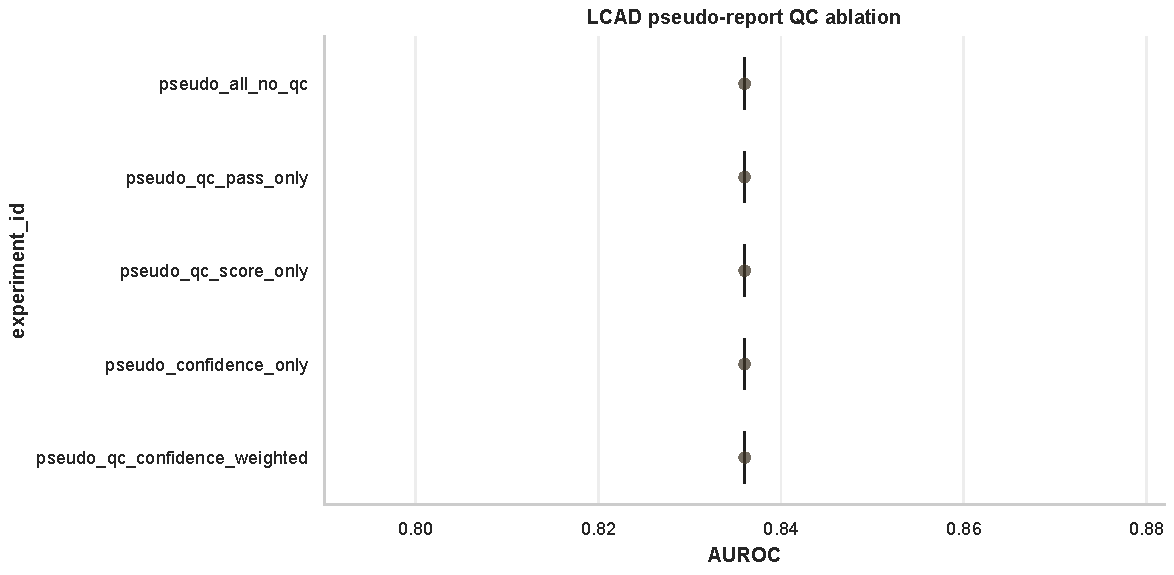
\includegraphics[width=0.82\linewidth]{final_Fig/fig_lcad_qc_ablation_barplot.pdf}
  \caption{Supplementary quality-control ablation for LCAD pseudo-report supervision. The analysis evaluates whether alternative pseudo-report filtering and weighting strategies materially alter downstream performance under the retrospective configuration; the separate failure-enriched stress test evaluates report-safety flagging rather than AUROC change.}
  \label{fig:qc_ablation}
\end{figure}

\section*{Section-level perturbation degradation profiles}
\begin{figure}[!htbp]
  \centering
  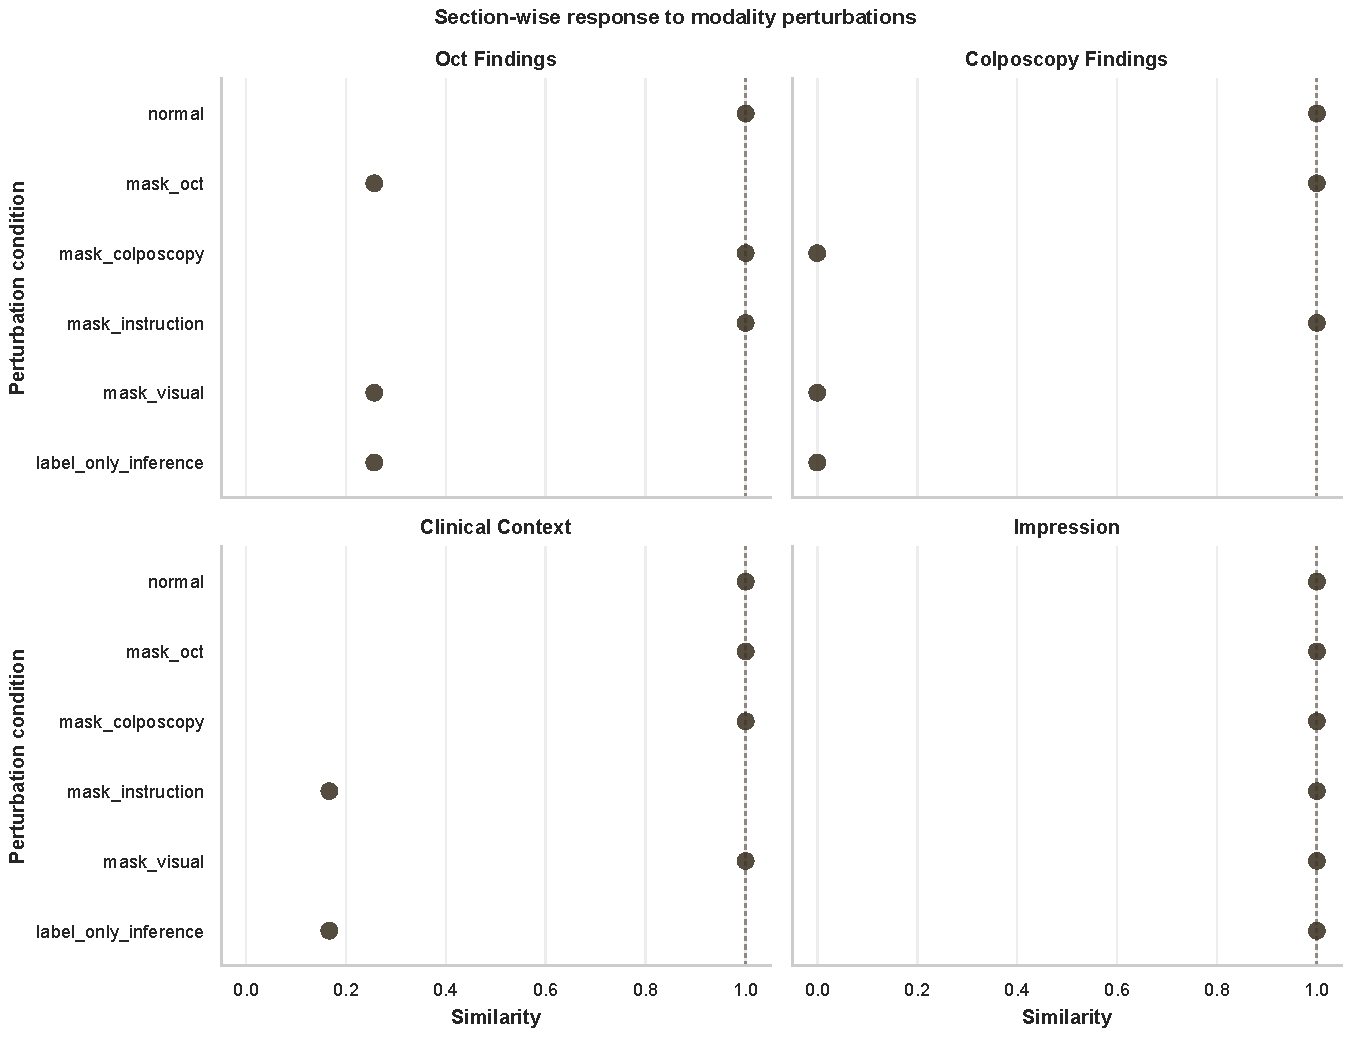
\includegraphics[width=\linewidth]{final_Fig/Figure3_modality_perturbation_lineplot.pdf}
  \caption{Supplementary section-level degradation profiles following modality-specific perturbations. The curves show whether disruption of a given input modality preferentially degrades the report section that should be grounded in that modality.}
  \label{fig:perturbation_lineplot}
\end{figure}

\section*{Risk-score displacement under perturbation}
\begin{figure}[!htbp]
  \centering
  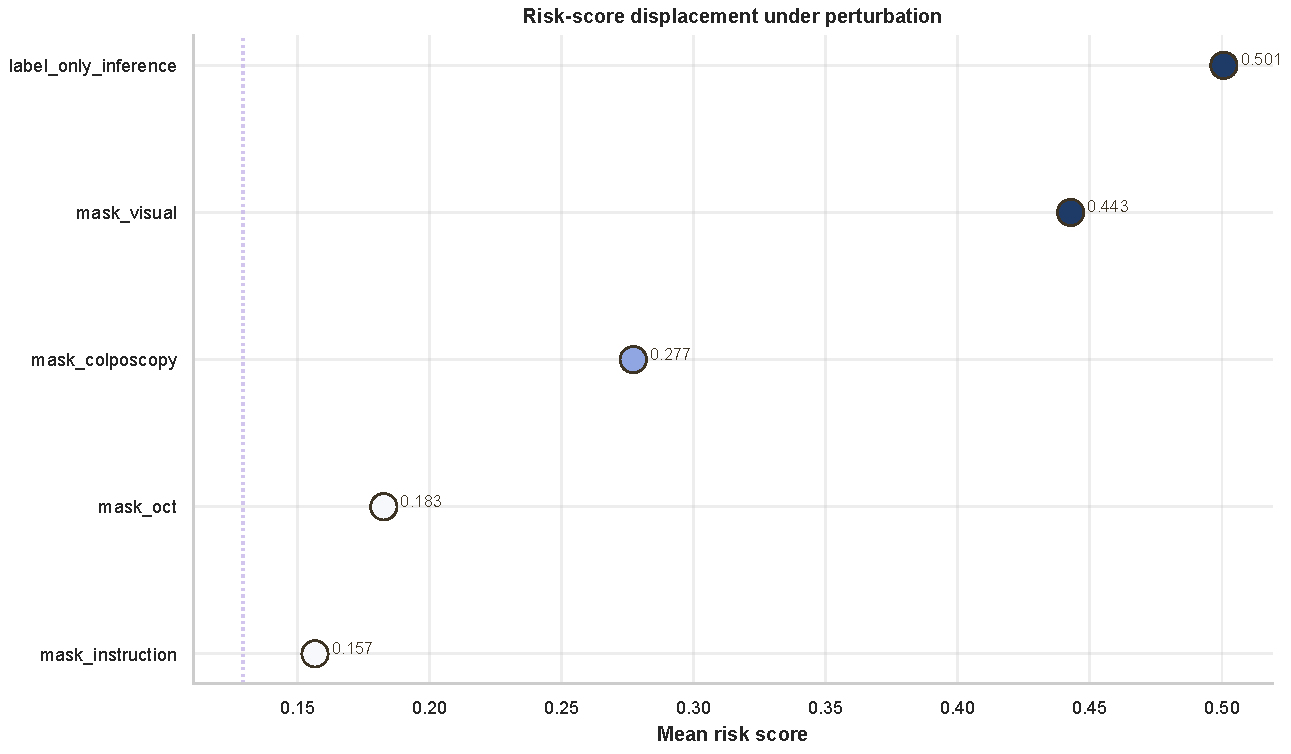
\includegraphics[width=\linewidth]{final_Fig/Figure3_risk_delta_stripplot.pdf}
  \caption{Supplementary risk-score sensitivity to report-generation perturbations. Absolute changes in predicted risk quantify the extent to which modality masking, modality shuffling, and label-only inference alter the model's diagnostic output.}
  \label{fig:risk_delta}
\end{figure}

\section*{Expanded perturbation sensitivity matrix}
\begin{figure}[!htbp]
  \centering
  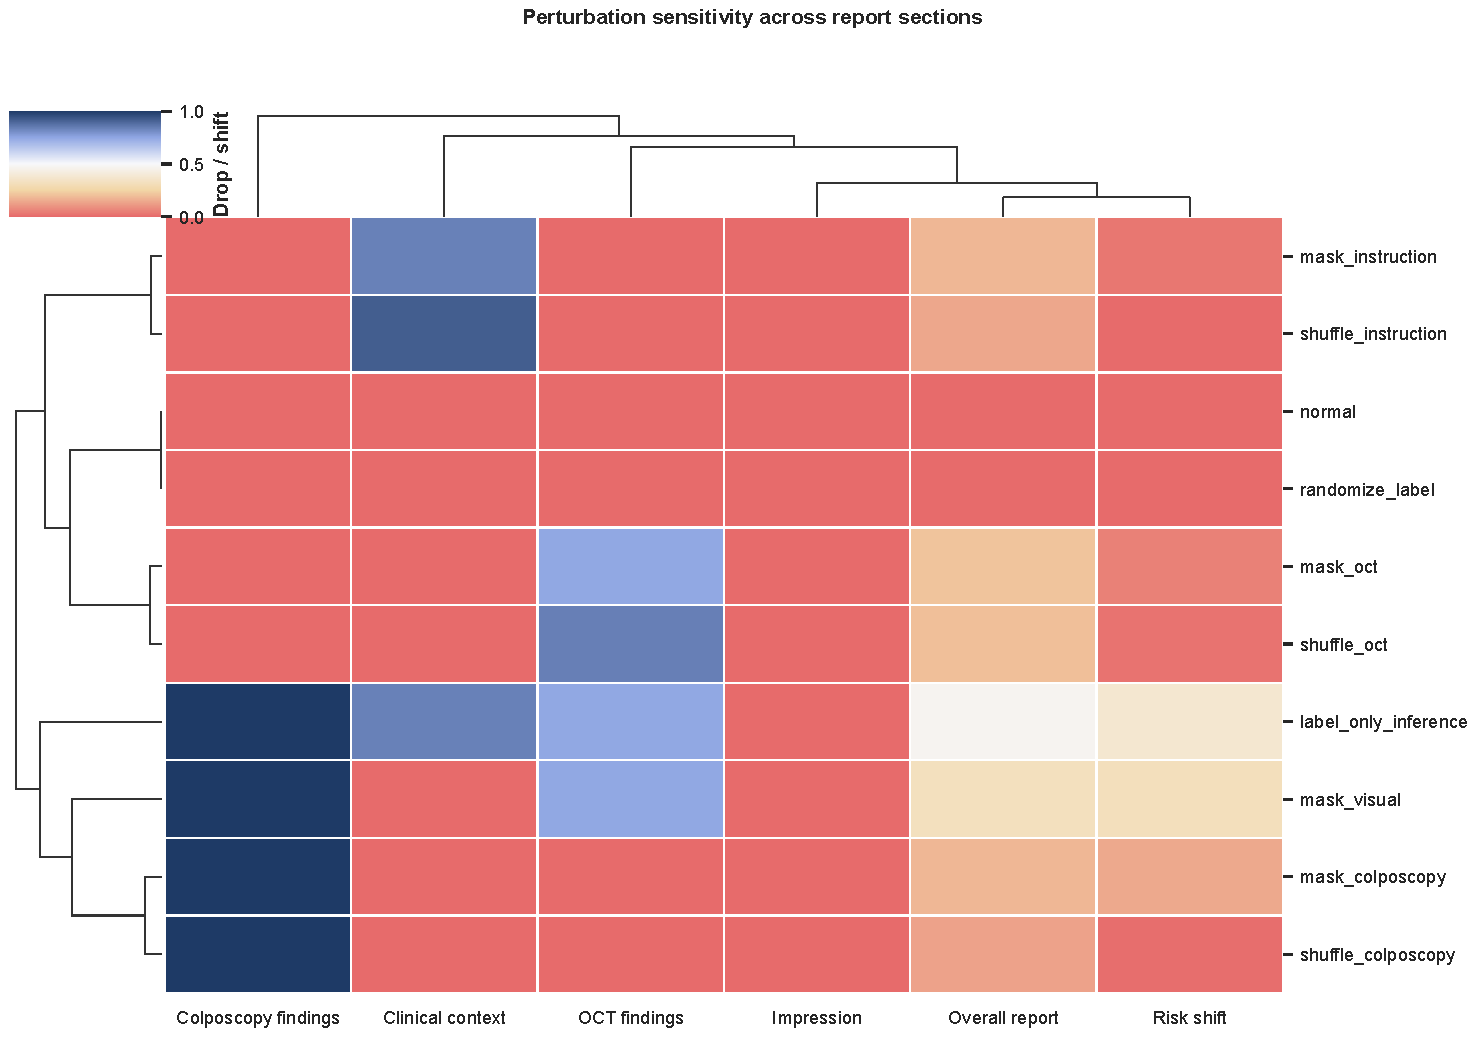
\includegraphics[width=\linewidth]{final_Fig/Figure_theme1_perturbation_sensitivity_matrix.pdf}
  \caption{Supplementary upgraded perturbation sensitivity matrix for Theme 1 cross-modal semantic alignment. The matrix consolidates section-level degradation, report-level degradation, risk shift, and specificity of the expected modality-section response.}
  \label{fig:theme1_perturbation}
\end{figure}

\section*{Strict leave-one-centre-out retraining}
\begin{table*}[!htbp]
  \centering
  \caption{Supplementary Table S2. Strict leave-one-centre-out retraining under the fixed quick-budget protocol.}
  \label{tab:s2_loco_strict_retrain}
  \scriptsize
  \begin{threeparttable}
  \resizebox{\linewidth}{!}{%
  \begin{tabular}{llrr}
    \toprule
    \textbf{Held-out centre} & \textbf{Model} & \textbf{$n$} & \textbf{AUROC} \\
    \midrule
    \multirow{3}{*}{Enshi} 
      & MOSAIC-RASA backbone                               & 61 & \textbf{0.702} \\
      & Real-report-only decoder                & 61 & 0.617 \\
      & Report generation without section alignment & 61 & \underline{0.697} \\
    \addlinespace[2pt]
    \multirow{3}{*}{Jingzhou}
      & MOSAIC-RASA backbone                               & 55 & 0.648 \\
      & Real-report-only decoder                & 55 & 0.315 \\
      & Report generation without section alignment & 55 & \textbf{0.704} \\
    \addlinespace[2pt]
    \multirow{3}{*}{Shiyan}
      & MOSAIC-RASA backbone                               & 79 & 0.500 \\
      & Real-report-only decoder                & 79 & 0.500 \\
      & Report generation without section alignment & 79 & 0.500 \\
    \addlinespace[2pt]
    \multirow{3}{*}{Wuhan Renmin}
      & MOSAIC-RASA backbone                               & 13 & 1.000 \\
      & Real-report-only decoder                & 13 & 1.000 \\
      & Report generation without section alignment & 13 & 1.000 \\
    \addlinespace[2pt]
    \multirow{3}{*}{Xiangyang}
      & MOSAIC-RASA backbone                               & 80 & \textbf{0.382} \\
      & Real-report-only decoder                & 80 & \textbf{0.382} \\
      & Report generation without section alignment & 80 & 0.370 \\
    \bottomrule
  \end{tabular}%
  }
  \begin{tablenotes}[flushleft]
    \footnotesize
    \item F1, sensitivity, and specificity were constant within the fixed quick-budget strict LOCO export and were omitted from the compact table. Strict LOCO is a stress test of centre-held-out retraining, not a definitive external-validation claim.
  \end{tablenotes}
  \end{threeparttable}
\end{table*}

\section*{Eval-only centre-shift audit using the global checkpoint}
\begin{table*}[!htbp]
  \centering
  \caption{Supplementary Table S2b. Eval-only LOCO using the global checkpoint.}
  \label{tab:s2b_loco_eval_only_global_ckpt}
  \scriptsize
  \begin{threeparttable}
  \resizebox{\linewidth}{!}{%
  \begin{tabular}{llrrrr}
    \toprule
    \textbf{\makecell[l]{Held-out centre\\($n$; label consistency)}} & \textbf{Model} & \textbf{AUROC} & \textbf{F1} & \textbf{Sensitivity} & \textbf{Specificity} \\
    \midrule
    \multirow{4}{*}{\makecell[l]{Enshi\\(288; 0.741)}} 
      & Real-report-only decoder            & 0.809 & 0.500 & 0.374 & \underline{0.944} \\
      & Simple concatenation fusion         & 0.624 & 0.480 & \underline{0.512} & 0.750 \\
      & LCAD without section alignment      & \textbf{0.863} & \textbf{0.636} & \textbf{0.527} & 0.939 \\
      & MOSAIC-RASA backbone                     & \underline{0.821} & \underline{0.522} & 0.466 & \textbf{0.895} \\
    \addlinespace[2pt]
    \multirow{4}{*}{\makecell[l]{Jingzhou\\(288; 0.587)}}
      & Real-report-only decoder            & 0.830 & 0.450 & 0.410 & 0.890 \\
      & Simple concatenation fusion         & 0.652 & 0.410 & 0.380 & 0.850 \\
      & LCAD without section alignment      & \textbf{0.877} & \underline{0.520} & \underline{0.511} & \underline{0.910} \\
      & MOSAIC-RASA backbone                     & \underline{0.848} & \textbf{0.540} & \textbf{0.620} & \textbf{0.930} \\
    \addlinespace[2pt]
    \multirow{4}{*}{\makecell[l]{Xiangyang\\(288; 0.648)}}
      & Real-report-only decoder            & 0.657 & 0.371 & 0.338 & \underline{0.896} \\
      & Simple concatenation fusion         & 0.606 & 0.340 & \underline{0.410} & 0.860 \\
      & LCAD without section alignment      & \textbf{0.864} & \underline{0.545} & 0.396 & \textbf{0.987} \\
      & MOSAIC-RASA backbone                     & \underline{0.850} & \textbf{0.553} & \textbf{0.513} & 0.920 \\
    \addlinespace[2pt]
    \multirow{4}{*}{\makecell[l]{Wuda\\(89; 0.955)}}
      & Real-report-only decoder            & 0.736 & 0.359 & 0.386 & \underline{0.850} \\
      & Simple concatenation fusion         & 0.548 & \underline{0.424} & \underline{0.412} & \underline{0.850} \\
      & LCAD without section alignment      & \textbf{0.901} & \textbf{0.970} & \textbf{1.000} & 0.375 \\
      & MOSAIC-RASA backbone                     & \underline{0.894} & \underline{0.936} & \underline{0.901} & \textbf{0.750} \\
    \addlinespace[2pt]
    \multirow{4}{*}{\makecell[l]{Shiyan\\(288; 0.566)}}
      & Real-report-only decoder            & 0.592 & 0.380 & 0.420 & \underline{0.868} \\
      & Simple concatenation fusion         & \underline{0.644} & 0.322 & 0.250 & 0.701 \\
      & LCAD without section alignment      & \textbf{0.747} & \underline{0.400} & 0.250 & 0.850 \\
      & MOSAIC-RASA backbone                     & \underline{0.735} & \textbf{0.580} & \textbf{0.650} & \textbf{0.910} \\
    \bottomrule
  \end{tabular}%
  }
  \begin{tablenotes}[flushleft]
    \footnotesize
    \item Eval-only LOCO is reported separately from strict LOCO retraining and is not pooled with strict LOCO results. Repeated $n$ and label-consistency values were merged into the centre column.
  \end{tablenotes}
  \end{threeparttable}
\end{table*}

\section*{Centre-wise LOCO heatmap}
\begin{figure}[!htbp]
  \centering
  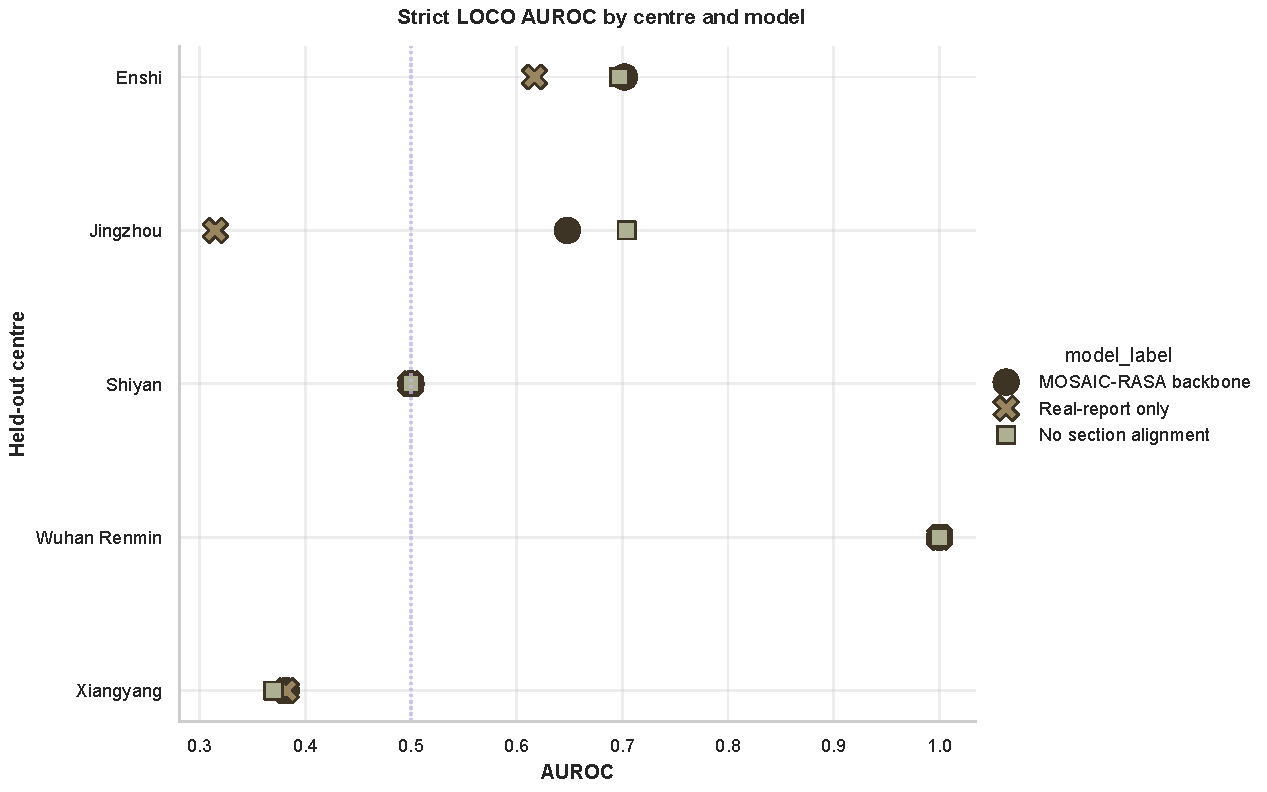
\includegraphics[width=1\linewidth]{final_Fig/fig_loco_heatmap.pdf}
  \caption{Supplementary leave-one-centre-out evaluation across participating centres. The panels summarise centre-wise AUROC patterns and strict LOCO performance, illustrating the extent of distribution shift under centre-held-out evaluation.}
  \label{fig:loco_heatmap}
\end{figure}

\section*{Strict LOCO forest plot}
\begin{figure}[!htbp]
  \centering
  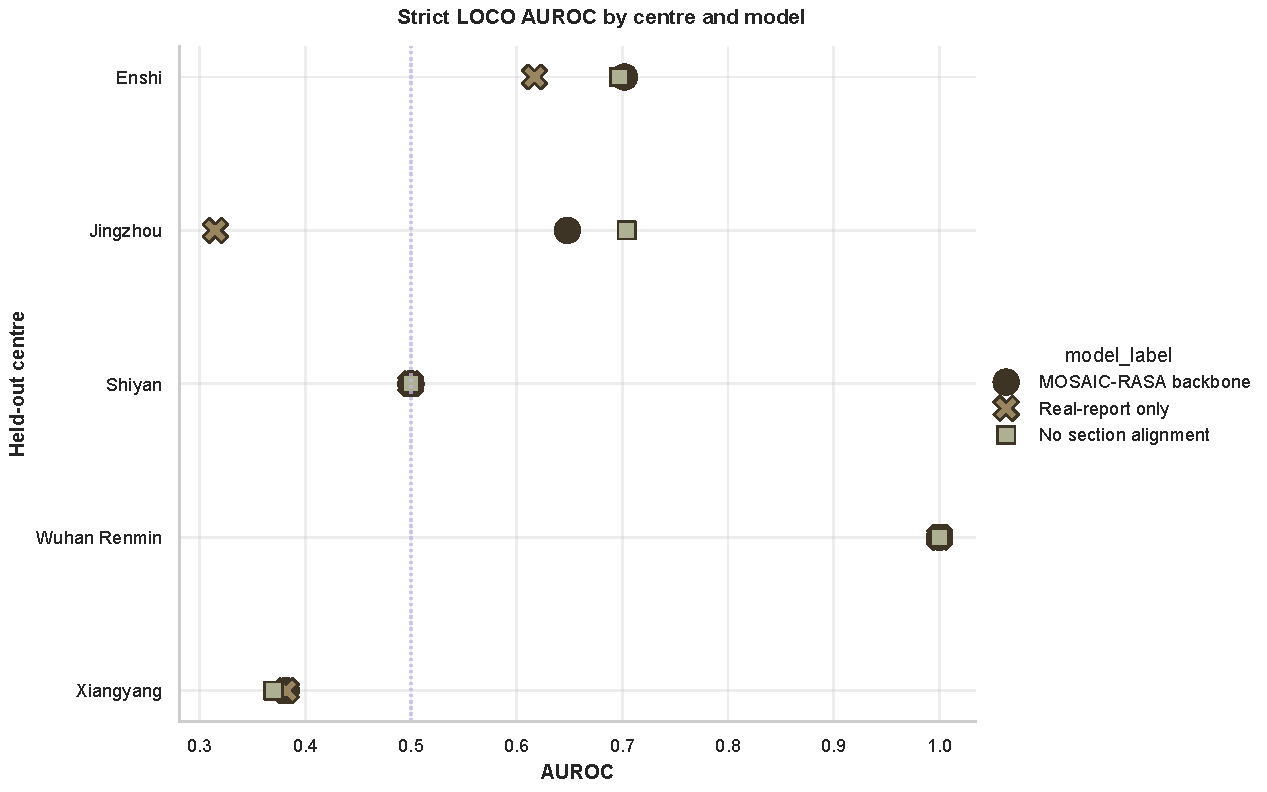
\includegraphics[width=\linewidth]{final_Fig/Figure4_loco_forest_catplot.pdf}
  \caption{Supplementary strict leave-one-centre-out behaviour under fixed quick-budget retraining. Centre-wise estimates characterise how MOSAIC-RASA backbone and comparator variants perform when each centre is held out during model fitting.}
  \label{fig:loco_forest}
\end{figure}

\section*{Multi-seed stability of backbone variants}
\begin{table*}[!htbp]
  \centering
  \caption{Supplementary Table S7. Multi-seed AUROC stability.}
  \label{tab:s7_multiseed_stability}
  \scriptsize
  \begin{threeparttable}
  \resizebox{\linewidth}{!}{%
  \begin{tabular}{lrrr}
    \toprule
    \textbf{Model} & \textbf{Mean AUROC} & \textbf{95\% interval} & \textbf{SD} \\
    \midrule
    MOSAIC-RASA backbone                    & \underline{0.776} & [0.773, 0.781] & 0.004 \\
    Report generation without section alignment & \textbf{0.780} & [0.767, 0.795] & 0.012 \\
    Real-report-only decoder                 & 0.667 & [0.656, 0.679] & 0.010 \\
    \bottomrule
  \end{tabular}%
  }
  \begin{tablenotes}[flushleft]
    \footnotesize
    \item The original metric-by-row table contained several constant rows. Across all seeds and models, mean F1 was 0.510, section completeness was 1.000, hallucination rate was 0.000, and label consistency was 0.641; the table therefore reports the variable stability metric, AUROC.
  \end{tablenotes}
  \end{threeparttable}
\end{table*}

\section*{Report-level safety indicators}
\begin{table*}[!htbp]
  \centering
  \caption{Supplementary Table S9. Report-level safety metrics.}
  \label{tab:s9_report_safety_metrics}
  \scriptsize
  \begin{threeparttable}
  \resizebox{\linewidth}{!}{%
  \begin{tabular}{lrrrrr}
    \toprule
    \textbf{Evaluated settings} & \textbf{\makecell{Missing-modality\\hallucination}} & \textbf{\makecell{Label-report\\contradiction}} & \textbf{\makecell{Recommendation\\contradiction}} & \textbf{\makecell{Section\\incompleteness}} & \textbf{\makecell{Any\\hallucination}} \\
    \midrule
    \makecell[l]{Real-report-only decoder;\\Simple concatenation fusion;\\No section alignment;\\MOSAIC-RASA backbone;\\Pseudo reports, no QC;\\QC-confidence weighted pseudo reports}
    & 0.000 & 0.847 & 0.000 & 0.000 & 0.000 \\
    \bottomrule
  \end{tabular}%
  }
  \begin{tablenotes}[flushleft]
    \footnotesize
    \item All evaluated settings had identical values in the current legacy rule-based safety table; duplicate rows were merged. The label-report contradiction scalar is definition-sensitive and is not used as a main-text safety endpoint. The refreshed failure-enriched QC stress test is reported as the primary report-safety filtering audit.
  \end{tablenotes}
  \end{threeparttable}
\end{table*}

\section*{Masking validation across centres}
\begin{table*}[!htbp]
  \centering
  \caption{Supplementary Table S10. Masking validation across agent settings and centres.}
  \label{tab:s10_masking_validation}
  \scriptsize
  \begin{threeparttable}
  \resizebox{\linewidth}{!}{%
  \begin{tabular}{llrrrrr}
    \toprule
    \textbf{Setting} & \textbf{Centre} & \textbf{$n$} & \textbf{Label consistency} & \textbf{ROUGE-L} & \textbf{BLEU} & \textbf{METEOR} \\
    \midrule
    \multirow{4}{*}{Label-only agent}
      & Enshi                  & 406 & 0.659 & 0.152 & 0.081 & 0.124 \\
      & Jingzhou               & 334 & 0.513 & 0.145 & 0.076 & 0.118 \\
      & Xiangyang              & 4   & 0.500 & 0.150 & 0.080 & 0.120 \\
      & Enshi--Jingzhou pooled & 740 & 0.593 & 0.149 & 0.079 & 0.121 \\
    \addlinespace[2pt]
    \multirow{4}{*}{\makecell[l]{Modality-only agent;\\Modality-plus-label agent}}
      & Enshi                  & 406 & \textbf{0.746} & \textbf{0.251} & \textbf{0.152} & \textbf{0.203} \\
      & Jingzhou               & 334 & 0.564 & 0.238 & 0.144 & 0.195 \\
      & Xiangyang              & 4   & \underline{0.750} & 0.245 & 0.148 & 0.200 \\
      & Enshi--Jingzhou pooled & 740 & 0.664 & \underline{0.246} & \underline{0.149} & \underline{0.198} \\
    \bottomrule
  \end{tabular}%
  }
  \begin{tablenotes}[flushleft]
    \footnotesize
    \item The modality-only and modality-plus-label agents produced identical values across centres; duplicate rows were merged.
  \end{tablenotes}
  \end{threeparttable}
\end{table*}

\section*{Scalability and runtime summary}
\begin{table*}[!htbp]
  \centering
  \caption{Supplementary Table S11. Scalability and runtime summary.}
  \label{tab:s11_scalability_runtime}
  \scriptsize
  \begin{threeparttable}
  \resizebox{\linewidth}{!}{%
  \begin{tabular}{lr}
    \toprule
    \textbf{Metric} & \textbf{Value} \\
    \midrule
    \multicolumn{2}{l}{\textbf{Cohort and image scale}} \\
    Total cases & 1,897 \\
    Total centres & 5 \\
    Total images & 137,591 \\
    OCT images & 129,030 \\
    Colposcopy images & 8,561 \\
    Mean images per case & 72.531 \\
    Median images per case & 123 \\
    Maximum images per case & 144 \\
    Real-report cases & 744 \\
    Pseudo-report cases & 1,153 \\
    Missing-report rate & 0.608 \\
    \addlinespace[2pt]
    \multicolumn{2}{l}{\textbf{Storage and checkpoint size}} \\
    Embedding storage & 47.349 MB \\
    Embedding files & 5,691 \\
    Publishable checkpoint size, MOSAIC-RASA backbone / pseudo-augmented / real-report-only & 79.882 MB \\
    Publishable checkpoint size, simple fusion / fusion plus section alignment & 79.879 MB \\
    \bottomrule
  \end{tabular}%
  }
  \end{threeparttable}
\end{table*}

\section*{Robustness figures for masking and seed stability}
\begin{figure}[!htbp]
  \centering
  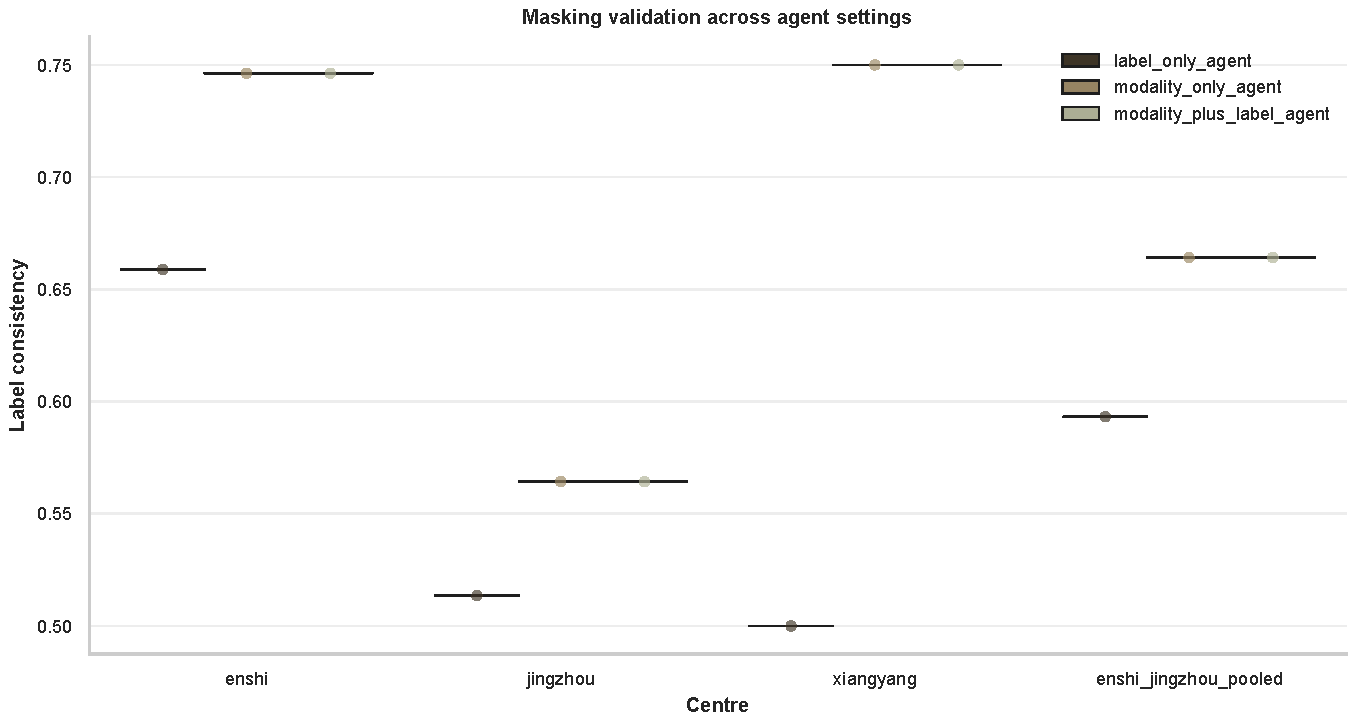
\includegraphics[width=\linewidth]{final_Fig/SupplementaryFigure_S1_masking_validation.pdf}
  \hfill
  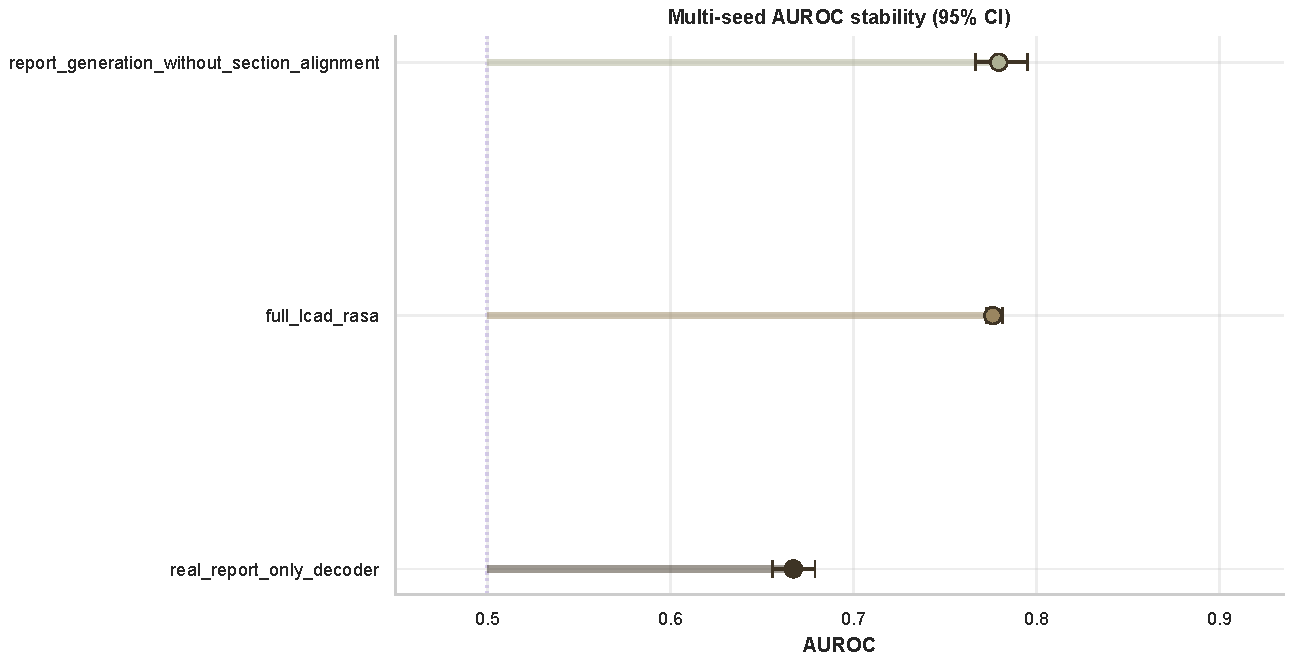
\includegraphics[width=\linewidth]{final_Fig/SupplementaryFigure_S3_multiseed.pdf}
  \caption{Supplementary robustness analyses. The panels summarise masking-validation behaviour and multi-seed stability, providing additional evidence on reproducibility and sensitivity of the retrospective pipeline.}
  \label{fig:supplementary_robustness}
\end{figure}
\end{document}
